\documentclass[a4paper,12pt,uplatex]{jsbook}

\newcommand{\V}[1]{\boldsymbol{#1}}
\def\thline{\noalign{\hrule height 1pt}}
\def\tvline{\vrule width 1pt}

\usepackage{makeidx}
\usepackage{amsmath}
\usepackage{amssymb}
\usepackage[dvipdfmx]{graphicx}
\usepackage{float}
\usepackage{bm}

\makeindex

\pagenumbering{roman}

\begin{document}
\title{平成27年度 修士論文\\
 \\
移動ロボットのための\\
不確かさを考慮した障害物回避行動の生成}
\author{鈴木勇矢\\
Chiba Institute of Technology}
\date{2020年2月x日}

% \maketitle
% \chapter*{謝辞}\addcontentsline{toc}{chapter}{謝辞}

本論文は, 著者が千葉工業大学大学院工学研究科未来ロボティクス専攻博士前期課程において行った研究をまとめたものです. 
本研究を進めるにあたって, ご指導を頂いた指導教員の千葉工業大学大学院工学研究科未来ロボティクス専攻 上田隆一准教授に, 感謝いたします. 
また, 副査としてご助言を頂いた, 米田完教授, ならびに林原靖男教授に感謝いたします. 
最後に, 研究などでお世話になりました同じ研究室の皆様, および未来ロボティクス専攻の先生方に感謝いたします. 


% \tableofcontents

%%% 本文 %%%
% 章のページの先頭は左側(奇数ページ)に来る
% \cleardoublepage
\pagenumbering{arabic}

% \chapter{序論} \label{chapter:introduction}


%%%%%%%%%%%%%%%%%%%%%%%%%%%%%%%%%%%%%%%%%%%%%%%%%%%%%%%%%%%%%%%%%%%%%%%%%%%%%%%%
\section{背景} \label{section:backglound}

\index{うえだ@上田} %消すとコンパイルできない
人間による操縦を必要とせず, 自律的に活動するロボットに対する社会の期待が高まっている. 
自律ロボットの活躍が期待される場所は多岐に渡り, 従来のロボットのように工場のラインだけでなく, 住宅や商業施設, あるいは被災地のような極限環境も含まれる. 
ロボットには様々な種類が存在するが, 中でも自律移動ロボットは, 病院内の搬送や空港の警備などの用途で, すでに社会実装されたものも多く存在する. 

これらの環境で移動ロボットが自律的に活動するためには, 自己位置や周辺環境の把握と行動計画を行う必要がある. 
実世界で活動するロボットは, 自身の位置を直接知ることはできない.  %あとで
したがって, 搭載したセンサを用いて自身の位置や周辺環境を把握する必要がある. 
そして, ロボットは把握した自己位置や環境の情報を頼りに, 目標地点へと移動するための行動を計画し動作する. 

しかしながら, 移動ロボットの活躍が求められている環境の多くは複雑で, 不確かな要素が多く存在する. 
人間の生活する空間は, 工業の組み立てラインのように不確かさや誤差がなるべく小さくなるように精密に構成されてはいない. 
また, センサが知覚できる情報には限りがありノイズが含まれているため, ロボットが環境の情報を完全に知覚することはできない. 
アクチュエータにおいても, 制御ノイズや消耗のような要因から誤差が存在し, モデル化やアルゴリズムの近似による誤差も存在する. 
したがって, ロボットが実世界で自律的に活動するためには, これら多くの不確かさに対処していく必要がある. 

不確かさを考慮するためには, 確率論に基づく方法が有効である. 
ロボティクスにおいて, 確率論を用いて不確かさに対処する試みは「確率ロボティクス(Probabilistic Robotics)」と呼ばれ, 盛んに研究が行われている\cite{thrun2005,上田2007prob}. 
確率ロボティクスは, ロボットの知覚と制御に確率・統計を駆使することで, ロボット技術において避けて通ることができない不確かさを陽に表現することを可能としている. 
移動ロボットにおいて重要な自己位置推定や行動計画についても, 不確かさを考慮した様々なアルゴリズムが提案されている. 

この確率論に基づく自己位置推定には, ベイズフィルタが有効であると示されている. 
確率ロボティクスでは, ロボットの自己位置を決定論的な一つの位置ではなく, 空間中における確率分布として表現する. 
ベイズフィルタによる自己位置推定では, ベイズの定理に基づき, 確率分布を逐次更新していく. 
この分布は信念分布と呼ばれ, ロボットが得られる情報をもとに, 主観的に自身の位置をどのように信じているかを表している. 

現在, 多くの移動ロボットにおいて, 確率論に基づく自己位置推定が取り入れられている. 
中でもとくに, Monte Carlo localization (MCL) という手法が多く利用されている\cite{dellaert1999, fox1999}. 
これは, ベイズフィルタによるロボットの自己位置推定を実装する方法の1つである. 
MCLでは, ロボットの信念分布を位置と姿勢からなる空間中に分布させた重みを持つ粒子(パーティクル)で近似的に表現する. 
これにより, ロボットの信念を複雑な確率分布として表現することを可能としている. 
同じくベイズフィルタを理論的背景としたカルマンフィルタによる自己位置推定では, 信念は正規分布でしか表現できない\cite{kalman1960}. 
対して, MCLでは一様や多峰性の分布などを表現することが可能であるため, 複雑な環境で活動することが求められる移動ロボットに適している. 
ロボット開発用のミドルウェアであるROSでは, LiDARと専有格子地図を用いたMCLによる自己位置推定のプログラムが, 標準のナビゲーションパッケージとして用意されており, 多くの開発者や研究者に利用されている\cite{quigley2009ros,roswiki_amcl}. 
また, 実環境において移動ロボットに自律移動を行わせる技術チャレンジであるつくばチャレンジでは, 多くのチームがLiDARと専有格子地図用いたMCLを用いている. 
\cite{夏迫2016つくばチャレンジ}
これらのことからも, MCLは実環境における自律移動ロボットの自己位置推定の手法として, 有効であることが分かる. 

現在, 様々な自律移動ロボットにおいて確率的な自己位置推定手法が取り入れられている一方で, 行動決定においては不確かさについて考慮されないことがある. 
一般的に多くの自律移動ロボットは, MCLやカルマンフィルタにより自身の位置を確率分布として推定する. 
そして, 最も確率の高い位置を自身が存在する真の位置だと仮定し, 行動計画を行う. 
しかし, このような方法では, ロボットの自己位置推定により得られた確率的な情報が, 行動決定に反映されない. 
ロボットは信念分布が大きい場合も, 分布が推定誤差が小さい場合も, 同様の行動を行うことになる. 
% たとえば, つくばチャレンジにおいて, 曲がり角で内側の段差にタイヤがははまり込みリタイアとなった例がある. (以前話で聞いただけなので参考となる文献を探す)

ロボット同様に, 実世界で活動する我々にとっても不確かさは避けることができない問題だが, 
人間や一部の動物は, 得られる情報が制限されている状況下でも, 適切な行動を選択する. 
たとえば, 人間は壁沿いを移動することで暗闇の中でも寝室に向かうことが可能であり, 
明るく視界に制限がないときとは異なる動作を行うことで, 不確かさに対処している. 
このように状況に合わせた自律的な行動をロボットに行わせるためには, 行動決定アルゴリズムで不確かさを考慮することが必要である. 


%%%%%%%%%%%%%%%%%%%%%%%%%%%%%%%%%%%%%%%%%%%%%%%%%%%%%%%%%%%%%%%%%%%%%%%%%%%%%%%%
\section{先行研究} \label{section:related works}

不確かさに応じた柔軟な行動決定をロボットに行わせることができると, 得られる情報が制限された状況下でもタスクを実行させることが可能となる. 
ロボット工学では, 部分観測マルコフ決定過程(POMDP)という枠組みで研究されているが, 計算量の観点から最適な解を導くことができないと知られている\cite{kaelbling1998}. 
そこで, 近似的にPOMDPを解く手法が複数提案されている. 

暗闇の中, 壁伝いに寝室へ向かうような行動については, Royらによって提案された手法によりロボットへと実装されている\cite{roy1999b}. 
この手法では, ロボットは事前に4次元の状態空間において行動計画が行われる. 
状態は, X-Y平面上ロボットの位置と方向に, 推定の不確かさの大きさを表すスカラー値を足した, 4つで表される. 
計画された行動には, 推定の不確かさを小さく保ちながらゴールへと向かう特性が現れた. 
この研究では, ロボットの自己位置推定は壁との距離を測定することで行われるため, ロボットは壁から大きく離れないようにゴールへと向かう動作を行った. 
この手法は, 沿岸航法(coastal navigation)と呼ばれる. 

Littmanらによって提案された$Q_{\rm MDP}$ value method\cite{littman1995}は, 事前の行動計画と観測の不確かさを分けて扱った. 
Q-MDP法では, 観測の不確かさを考慮せずに, マルコフ決定過程の問題としてロボットの行動を事前に計画し, 
実際にロボットが行動を決定するときに, 観測の不確かさを考慮する. 
事前に計画した行動と現在の信念の確率分布から, 各行動に対する期待値計算を行い, 最も良い行動を選択する. 

$Q_{\rm MDP}$ value methodは, Uedaらによって実際のロボットへと実装された\cite{ueda2003iros}. 
RoboCupの四足歩行リーグのゴールキーパーのロボットへと適用され, 有効性が示された. 

Uedaによって提案されたPFC法では, 移動ロボットがゴールを探索するような動作を可能にしている\cite{ueda2015}. 
この手法では, $Q_{\rm MDP}$ value methodの行動評価の式に変更を加えることで, ゴールに近いパーティクルが行動決定に及ぼす影響を大きくする. 
これにより, ロボットは自身の位置がほぼ分からない状況から, パーティクルにより近似された信念を徐々にゴールに流し込むような動作を行う. 
分布が徐々にゴールに吸い込まれるように移動していき, ロボットが分布の中にいる場合, ロボットもその流れに従いゴールへと到達する. 
また, ゴール付近のパーティクルが行動決定に及ぼす影響の大きさを変更した際に, 
$Q_{\rm MDP}$ value methodで問題となっていた, ローカルミニマムによる行動の停滞が起こる頻度が低下することについても示されている\cite{ueda2018searching}. 

PFC法は, 障害物が存在しない空間において, 自己位置推定が極めて不確かな移動ロボットのナビゲーションに有効であることが, シミュレーション実験において示されている. 
しかし, 障害物が存在する環境での動作については, 有効性は確認されていない. 
PFC法では, ゴール付近のパーティクルが行動決定に及ぼす影響を大きくする一方で, 
ゴールから遠いパーティクルや障害物内に存在するパーティクルは, 軽視されることになる. 
つまり, ロボットが障害物を回避しようとする行動は反映されにくいという性質がある. 
一般的に, 自律移動ロボットが活動することが求められている環境には, 動的なものや静的なものを含め, 多くの障害物が存在する. 
移動ロボットのナビゲーションでは, 障害物の回避について考えることが必要であると言える. 


\section{目的}
そこで本研究では, 自己位置推定の不確かさを考慮した障害物の回避行動を自律移動ロボットに行わせるための手法を提案する. 
PFC法に変更を加えることで, 信念を近似するパーティクル全体が障害物を回避するような動作を生成する. 
これにより, 自律移動ロボットに自己位置推定の不確かさを考慮した障害物回避の行動をとらせつつ, ゴールを探索するような動作を行わせることを可能にする. 
また, その有効性について通常のPFC法と比較することで検証する. 


%%%%%%%%%%%%%%%%%%%%%%%%%%%%%%%%%%%%%%%%%%%%%%%%%%%%%%%%%%%%%%%%%%%%%%%%%%%%%%%%
\section{本論文の構成}
まず, 第\ref{chapter:introduction}章では, 本研究の背景と先行研究を述べ, 目的を設定した. 
第\ref{chapter:localization}章では, ロボットの状態推定について述べる. 
第\ref{chapter:pomdp}章では, 不確かさを考慮したロボットの行動決定について述べ, 
第\ref{chapter:method}章では, 提案する手法について述べ, 
第\ref{chapter:evaluate}章では, 提案手法をPFC法と比較し評価する. 
最後に第\ref{chapter:conclusion}章で, 本論文の結論を述べる. 


% \begin{figure}[ht]
%   \begin{center}
%     \includegraphics[width=10cm, ]{figs/image.png}
%   \end{center}
% \end{figure}

% \chapter{移動ロボットの自己位置推定} \label{chapter:localization}

%%%%%%%%%%%%%%%%%%%%%%%%%%%%%%%%%%%%%%%%%%%%%%%%%%%%%%%%%%%%%%%%%%%%%%%%%%%%%%%%
本章では, Bayesian Filterによる移動ロボットの自己位置推定について定式化する. 
また, Bayesian Filterの実装方法の1つであるMonte Carlo Localization (以下MCL)について述べる. 
本論文においても, 移動ロボットの自己位置推定にはMCLが利用されるものとする. 

% Bayesian Filterによる状態推定では, ロボットはセンサにより得た情報や自身の制御出力の履歴から, 状態空間$\chi$内での現在の状態を確率的に推定する. 
% ロボットの状態を表すパラメータについては様々存在するが, 自己位置推定ではロボットの姿勢(位置と向き)を推定することを目的としている. 
% 本論文では, 二次元平面を低速で移動する対向二輪型のロボットを想定し, ロボットの二次元平面上における位置$x, y$と向き$\theta$をあわせた3次元の状態$(x, y, \theta)$の推定について扱う. 


%%%%%%%%%%%%%%%%%%%%%%%%%%%%%%%%%%%%%%%%%%%%%%%%%%%%%%%%%%%%%%%%%%%%%%%%%%%%%%%%
\section{Bayesian Filterによる自己位置推定}

% Bayesian Filterによる自己位置推定では, 式(\ref{bayes theorem})に示すベイズの定理を用いて, 移動ロボットの位置を確率的に推定する. 
% ベイズの定理は, 事象$a, b$が起きる確率をそれぞれ$p(a), p(b)$としたときに, 
% \begin{equation}
% \label{bayes theorem}
%   y = a
% \end{equation}



%%%%%%%%%%%%%%%%%%%%%%%%%%%%%%%%%%%%%%%%%%%%%%%%%%%%%%%%%%%%%%%%%%%%%%%%%%%%%%%%
\section{Monte Carlo Localization (MCL)}

Monte Carlo Localization (MCL)は, Bayesian Filterを理論的背景としたロボットの自己位置推定手法の実装方法の1つである. 
MCLでは, 表現したい任意の空間上$\mathcal{X}$上に存在する確率密度関数を, 空間上に散布した標本により表現することで, ロボットの姿勢を確率的に推定する. 
この標本はパーティクル(粒子)と呼ばれ, ロボットの信念分布を表す確率密度関数$b_t(\bm{x})$を近似するように配置される. 
パーティクルはそれぞれパラメータとしてロボットと同次元の姿勢$\bm{x}$と重み$w$の情報を持っており, $N$個のパーティクルの集合は
\begin{equation}
\label{particles}
  \Xi_{t} = {\xi^{(i)}_{t} = (\bm{x}^{(i)}_{t}, w^{(i)}_{t} |i = 1,2,\dots,N) }
\end{equation}
のように定義される. 
基本的に全パーティクルの重みの合計は, 常に
\begin{equation}
\label{weight_sum}
  \sum_{i=1}^{N}w^{(i)}_{t}=1
\end{equation}
を保つように実装される. 

ロボットの状態を表すパラメータについては様々存在するが, 自己位置推定ではロボットの姿勢(位置と向き)を推定する. 
本論文では, 二次元平面を低速で移動する対抗二輪型の移動ロボットを想定し, ロボットの二次元平面上における位置$(x, y)$と向き$\theta$をあわせた3次元の状態$\bm{x} = (x, y, \theta)$の推定について扱う. 
したがって, ロボットの姿勢と同様に, パーティクルの姿勢はそれぞれ$\bm{x}^{(i)} = (x^{(i)}, y^{(i)}, \theta^{(i)})$となる. 

% MCLには大きな利点が2つある. 
% 1つ目の利点は, \ref{section:backglound}でも述べたとおり, 多様な確率分布を表現できることである. 
% もう1つの利点は, アルゴリズムが簡単なことである. 
% したがって, 比較的容易に実装することが可能である. 

MCLのアルゴリズムは, 主に次の4ステップからなる. 
2から4を繰り返し行うことで逐次ロボットの姿勢を推定する. 
\begin{enumerate}
  \item 初期化
  \item 動作による更新
  \item 計測による更新
  \item リサンプリング
\end{enumerate}

% ロボットの真の姿勢を$\bm{m}^{*}$とすると, ある時刻$t$におけるロボットの信念分布は$bel_{t}$と表現され, 
% 本章のはじめで述べたとおり, 本論文では移動ロボットの姿勢$\bm{x} = (x, y, \theta)$を推定することを想定したMCLを述べる. 
% 各パーティクルはある時刻$t$におけるロボットの状態の具体的な事例であり, 真の状態に対する1つの仮説と考えることができる. 

% 標本はパーティクルと呼ばれる
% パーティクルはロボットの信念分布を近似するようにばらまかれる
% パーティクルは式で表現される
% 真の姿勢が存在する確率をしめす. 
% これをパーティクルで表現すると


%%%%%%%%%%%%%%%%%%%%%%%%%%%%%%%%%%%%%%%%
\subsection{初期化}

初期化のステップでは, パーティクルの初期化を行う. 
N個のパーティクルの初期姿勢$\bm{x}^{(i)}$を決定し, 重み$w^{(i)}$を$\frac{1}{N}$とする. 
パーティクルのばらまき方は, ロボットの初期の信念分布に従うように行う. 
一般的には, 以下のようなパーティクル初期姿勢の決定方法が用いられる. 

ロボットを人間が自由に配置する場合など, 初期姿勢が予め分かっている場合は, ロボットの信念分布をロボットが存在すると考えられる位置を平均とした正規分布と考え, 
パーティクルの初期姿勢$\bm{x}^{(i)}$を平均$\mu$, 分散$\Sigma$の正規分布に従うように決定する. 
本論文における移動ロボットの自己位置推定では, 状態$\bm{x}^{(i)}$が位置と向きからなる3次元のため, $\mu$と$\Sigma$はそれぞれ3次元ベクトル, $3\times3$の分散共分散行列として扱う. 
多くの場合$\mu$と$\Sigma$はヒューリスティックに決定する. 

一方, ロボットの初期位置が完全に不明なとき, ロボットの初期信念分布は状態空間$\mathcal{X}$全体の一様分布と考えられる. 
その場合は, パーティクルの姿勢は一様分布に従うように配置する. 

% MCLは, ロボットの制御出力や移動量, センサに含まれるノイズに頑健な推定が行える. 
% しかし, 想定を上回るノイズが混入した場合に, ロボットの真の姿勢$\bm{x}^{(*)}$とパーティクルの分布$\Xi$が大きく乖離することがある. 
% MCLでは, パーティクルの分布がロボットの真の位置$\bm{x}^{*}$がから大きく離れることがある. 
% このようなロボットの真の姿勢の周辺にパーティクルが存在しない状態は, 「誘拐状態」と呼ばれる. 
% 誘拐状態となったとき, 一般的にはふたたびパーティクルが真の姿勢周辺に戻ることは少ないとされ, 推定が大きく誤った状態が続く. 
% そこで, 融解状態から回復するための研究が複数行われている. 
% 本論文では, ロボット


%%%%%%%%%%%%%%%%%%%%%%%%%%%%%%%%%%%%%%%%
\subsection{動作による更新}

動作による更新のステップでは, Bayesian Filterにおける予測ステップを, 各パーティクルに対して行う. 
移動ロボットの状態遷移にはノイズが伴うため, 同様の制御入力でも試行ごとに異なる状態遷移結果となる. 
したがって, ロボットが動作すると信念分布が広がることになる. 
この広がった信念分布を表現するように, パーティクルの分布を更新する. 
各パーティクルの状態をロボットの動作モデル
ロボットの状態遷移確率$p(\bm{x} | \bm{x}_{t-1}, \bm{u}_{t})$とすると, 
動作後の各パーティクルの姿勢は
\begin{equation}
\label{particle trans prob}
  \bm{x}^{(i)}_{t} \sim p(\bm{x} | \bm{x}_{t-1}, \bm{u}_{t})
\end{equation}
のように更新される. 


%%%%%%%%%%%%%%%%%%%%%%%%%%%%%%%%%%%%%%%%
\subsection{計測による更新}

計測による更新のステップでは, Bayesian Filterにおける計測更新ステップを行う. 
センサにより得られた情報が, 各パーティクルの状態で得られる確率を計算し, 重み$w^{(i)}$を更新する. 
重みの更新はベイズの定理を用いて
\begin{equation}
\label{weight}
  w^{(i)}_{t} = q(\bm{z}_{t} | \bm{x}^{(i)}_{t}) \hat{w}^{(i)}_{t}
\end{equation}
のように計算される. 
尤度関数$q(z_{t} | \bm{x}^{(i)}_{t})$は, 使用するセンサの観測モデルをもとに決定する. 

現在, 移動ロボットの自己位置推定のために, LiDARと呼ばれる光センサによる測距センサや, RGB-Dカメラが広く利用されている. 
これらのセンサを自己位置推定位に用いるロボットは, 条件が揃えば非常に正確な推定を行うことが可能である. 
しかし, 本論文では移動ロボットの状態推定が不確かなときに有効となるような行動決定の手法を提案することを目的としている. 
したがって, 移動ロボットが曖昧にしか状態推定を行えない状況を想定するために, ロボットはこれらのセンサを搭載していないものとする. 

代わりに, ロボットはタスクの終了を検知することができるものとする. 
この仮定は, \ref{chapter:method}章で述べる提案手法, およびその先行研究となるPFC法で必要となる. 
ロボットは, 自身がゴールに到達したか否かを各ステップごとに知ることができ, その情報を計測による更新に用いることができるものとする. 

%%%%%%%%%%%%%%%%%%%%%%%%%%%%%%%%%%%%%%%%
\subsection{リサンプリング}
リサンプリングステップでは, パーティクルを再配置し重みを均一にする. 
再配置するパーティクルは, 重みに従った確率で選択される. 
重みの小さいパーティクルを間引き, 重みの大きいパーティクルの位置に多くのパーティクルを配置する. 
この操作により, 一箇所に重みが偏り続け推定の精度が下がることを防ぐ. 

パーティクルの選択(サンプリング)にはいくつかの手法が存在する. 
本論文では, 系統抽出法によるリサンプリングを用いる. 

% \chapter{不確かさを考慮した行動決定}

本章では、不確かさを考慮した行動決定について述べる。
まず、状態が既知のロボットの最適な行動決定を扱う枠組みである「マルコフ決定過程」について述べる。
その後、ロボットの状態が不確かにしか分からない状況での最適な行動を扱う枠組みである「部分観測マルコフ決定過程」について述べる。
最後に、「部分観測マルコフ決定過程」を近似的に解く手法について、いくつかあるうち、本研究と関連のあるQ-MDP法およびPFC法について述べる。


%%%%%%%%%%%%%%%%%%%%%%%%%%%%%%%%%%%%%%%%%%%%%%%%%%%%%%%%%%%%%%%%%%%%%%%%%%%%%%%%
\section{ロボットの行動決定}
本節では、ロボットの行動決定について考える。
本論文で扱うような移動ロボットの行動決定は、現在のロボットの位置から目的地までの最短経路を算出して移動する、「経路計画問題」として扱われる。
ダイクストラ法やA*法、人工ポテンシャル法といった多くの手法が提案されており、現在でも研究が行われている。
一般的にロボットの経路計画問題では、ロボットの観測や移動は決定論的なもとのして扱われ、経路の算出が行われる。

しかし、これまで述べたとおり、移動ロボットは多くの不確かさを有している。
移動ロボットに最短の経路を算出して移動するだけでなく、これらの不確かさを考慮した上でさらに知的な動作を行わせる方法について考える必要がある。
たとえば、人間であれば、最短ではあるが危険でゴールに到達できる可能性が低い道よりも、多少遠回りではあるが高確率で安全にゴールできる道を選択するような、
「急がば回れ」が有効な場合も存在する。
あるいは、自身の位置が正しく把握できていない場合に、安全を優先し全く動かないでいるよりも、
多少の危険を冒しとりあえず行動してみてタスク達成を目指す方が有効であるような場合も考えられる。

このような知的な行動を、単純に経路計画問題として考えることは困難である。
そこで本章では、ロボットの移動と経路計画について、
より一般化した枠組みである(有限)マルコフ決定過程および部分観測マルコフ決定過程について述べる。

%%%%%%%%%%%%%%
%%%%ロボットの不確かさは大きく分けて、動作に関するものと観測に関するものの2つに分類できる。


%%%%%%%%%%%%%%%%%%%%%%%%%%%%%%%%%%%%%%%%%%%%%%%%%%%%%%%%%%%%%%%%%%%%%%%%%%%%%%%%
\section{マルコフ決定過程} \label{section:mdp}
本節では、移動ロボットの現在の自己位置$\bm{x} \in \mathcal{X}$が既知という前提での行動決定についての定式化を行う。
このような問題は、マルコフ決定過程(Markov decision process, MDP)という枠組みで議論される。
時間やロボットの状態等を連続系ではなく離散系で考える場合は、有限マルコフ決定過程と呼ばれる。
% また、本論文では、とくに断りがない場合MDPは離散系の有限マルコフ決定過程のことを指す。

%%%%%%%%%%%%%%%%%%%%%%%%%%%%%%%%%%%%%%%%
\subsection{状態と終端状態}
章\ref{chapter:localization}で述べたものと同様に、
状態変数$x,y,\theta$からなる状態空間$\mathcal{X}$を定義する。
ロボットは自身の現在の状態ベクトル$\bm{x} \in \mathcal{X}$が分かっているものとし、観測の不確かさについては考慮しない。

ロボットのタスクには必ず終わりがあるとし、
ロボットの状態が、事前に定めたある状態になったときをタスクの終了とする。
このタスクが終了する状態は、終端状態と呼ばれ、終端状態の集合は$\mathcal{X}_f \subset \mathcal{X}$と表現される。
終端状態は、移動ロボットの経路計画問題における、ゴールや目標地点などのロボットが目指すべき望ましい状態だけでなく、陥りたくない状態も含まれる。

%%%%%%%%%%%%%%%%%%%%%%%%%%%%%%%%%%%%%%%%
\subsection{行動と状態遷移}
ロボットは有限子の制御指令の中から、一つを選択することで動作する。
MDPではこの制御指令のことを行動と呼ぶ。
ロボットの行動はm種類存在し、行動の集合は、
\begin{equation}
\label{action}
  \mathcal{A} = \{ a_{1}, a_{2}, \ldots , a_{m} \}
\end{equation}
と表現される。

時間は離散的に表現され、タスクの開始からは終わりまでは${0,1,2,\ldots,t_{f}} \equiv T$と定義される。
ロボットが最初に行動を選択する時刻を$t=0$とし、行動が実行されるたびに$t=1,2,\ldots$と次のステップへと進んでいく。
ロボットが終端状態に入りタスクが終了する時刻を$t_{f}$とする。
$t_{f}$は固定ではなく、タスク達成までにかかった時間により異なる。
また、「時刻$t-1$の状態」、「時刻$t$に遷移するために選択された行動」、「時刻$t$の状態」をそれぞれ$\bm{x}_{t-1}, a_{t}, \bm{x}_{t}$と表現する。
しかし、MDPで扱うシステムは時不変であるため、多くの場合$t$の具体的な値は重要でははない。
したがて、今後はこれらをそれぞれ$\bm{x}, a, \bm{x}^{'}$と表記する。

ロボットの状態$\bm{x}$は、ある行動$a$により状態$x^{'}$へと遷移する。
状態の遷移にはノイズが含まれているものとし、状態と行動が同一の$(\bm{x}, a)$であっても、事後状態$\bm{x}^{'}$は各試行ごとに異なる。
ロボットの状態遷移は、マルコフ性を持ち、
\begin{equation}
\label{trans prob}
  \bm{x} \sim p(\bm{x} | \bm{x}_{t-1}, \bm{u}_t) (t=1,2,\ldots,t_{f})
\end{equation}
に従うものとする。
また、ロボットが$\bm{x}$から行動$a$により$\bm{x}^{'}$に遷移する確率を$p^{a}_{\bm{x}\bm{x}^{'}}$と表現する。
この確率$p^{a}_{\bm{x}\bm{x}^{'}}$が、$\bm{x}, a, \bm{x}^{'}$のあらゆる組に対して既知であり、時不変であると仮定する。

%%%%%%%%%%%%%%%%%%%%%%%%%%%%%%%%%%%%%%%%
\subsection{報酬} \label{subsection:reward}
状態$\bm{x}$で行動$a$を行った場合に、状態が$\bm{x}^{'}$に遷移した際に、その状態遷移に対して報酬を与える。
たとえば、移動ロボットではこの報酬は、行動一回ごとに消費する電力や時間などを設定する。
この報酬は、一つの実数値とし、$r^{a}_{\bm{x}\bm{x}^{'}} \in \mathbb{R}$と表現される。
評価の基準が多次元的の場合も、一つの実数となるように一元化し評価を行う。

%%%%%%%%%%%%%%%%%%%%%%%%%%%%%%%%%%%%%%%%
\subsection{評価}
ロボットがある状態$\bm{x}$からある終端状態$\bm{x}_{f} \in \mathcal{X}_{f}$に到達するまでの一連の状態遷移に対して評価を与える。
評価は、
\begin{equation}
\label{evaluation}
  J( \bm{x}_{0:t_{f}}, a_{1:t_{f}} ) = \sum^{t_{f}}_{t=1} r^{a}_{\bm{x}\bm{x}^{'}} + V(\bm{x}_{t_{f}})
\end{equation}
で定義される評価値の大きさで行う。
$r^{a}_{\bm{x}\bm{x}^{'}}$は、項\ref{subsection:reward}で述べた報酬である。
$V(\bm{x}_{t_{f}})$は終端状態の価値とし、事前に目的に応じて与えられるものとする。
ロボットが目指すゴールや目標地点とする場合、$0$を設定する。
逆に、ロボットがその状態になった場合タスクが失敗として終了するような、絶対に陥ってほしくない状態として設定する場合、非常に小さい値を設定する。

本論文では、この評価値$J$を最大化する一連の状態遷移を、最適な制御とする。
状態遷移にはノイズが伴うため、同じ姿勢$\bm{x}_{0}$から常に最適となるような行動をとったとしても、試行ごとに評価値$J$は異なる。
そのため、ある状態から終端状態までの一連の状態遷移に対する評価$J$は、期待値として考える。

%%%%%%%%%%%%%%%%%%%%%%%%%%%%%%%%%%%%%%%%
\subsection{最適方策}
ある状態における、Jの期待値を最大化するための行動を与える関数
\begin{equation}
\label{policy}
  \Pi : \mathcal{X} \rightarrow \mathcal{A}
\end{equation}
を定義する。
この関数$\Pi$は最適方策と呼ばれる。
最適方策$\Pi$が決まると、任意の状態$\bm{x}$でロボットが取るべき行動は、
\begin{equation}
\label{oprimal action}
  a = \Pi(\bm{x}) \;\;\;\; (\forall \bm{x} \in \mathcal{X})
\end{equation}
と自動的に決まる。

%%%%%%%%%%%%%%%%%%%%%%%%%%%%%%%%%%%%%%%%
\subsection{最適価値関数}
また、ある状態に対して評価値の期待値$J$を与える関数
\begin{equation}
\label{value function}
  V : \mathcal{X} \rightarrow \mathbb{R}
\end{equation}
は、最適価値関数と呼ばれる。
$V(\bm{x})$は、$\bm{x}$が初期の状態でも、タスクにおける途中の状態でも変わらない。
終端状態の価値$V(\bm{x}_{t_{f}})$は、この最適価値関数に含まれる。


%%%%%%%%%%%%%%%%%%%%%%%%%%%%%%%%%%%%%%%%%%%%%%%%%%%%%%%%%%%%%%%%%%%%%%%%%%%%%%%%
\section{部分観測マルコフ決定過程}
本節では、移動ロボットの現在の状態が不確かな中での行動決定について述べる。
このような問題は、部分観測マルコフ決定過程(partially observable Markov decision process, POMDP)という枠組みで研究が行われている。

POMDPがMDPと異なる点は、ロボットが真の状態が分かっていないという点にある。
ロボットはMDP同様、評価値$J$を最小化するように終端状態にたどり着くことを目的とする。
しかし、ロボットの姿勢$\bm{x}$が未知であるため、最適方策$\Pi(\bm{x})$を使用することができない。
したがって、$\bm{x}$の代わりにその場で得られる情報をもとに行動を決定する必要がある。
ロボットがこれまで行ってきた行動の履歴$a_{1:t}$、それまでに得た観測の情報$z_{1:t}$、およびそれまでに得た報酬の履歴$r_{1:t}$から決定される方策は
\begin{equation}
\label{policy pomdp}
  a_{t+1} = \Pi_{\rm POMDP} (a_{1:t}, \bm{z}_{1:t}, r_{1:t})
\end{equation}
と定義される。

ロボットが行動を決定するとき、その時点での状態推定の不確かさを考慮したい場合、関数
\begin{equation}
\label{policy belief}
  a_{t+1} = \Pi_{\rm b} (b_{t})
\end{equation}
を考えればよいことになる。
この関数は、ロボットの姿勢を状態とするのではなく、ロボットの信念分布自体をひとつの状態としてみなし、
とるべき行動をロボットの現在の信念分布から決定する。
状態としてみなされる信念分布は、信念状態と呼ばれる。

このように信念の分布をひとつの状態とみなすことで、POMDPの問題をMDPの問題として考えることができる。
信念状態を用いることでPOMDPをMDPとして考える方法は、belief MDPと呼ばれる\cite{kaelbling1998}。
しかし、信念状態の数は非常に膨大であり、最適方策を得ることは通常不可能とされている。


%%%%%%%%%%%%%%%%%%%%%%%%%%%%%%%%%%%%%%%%%%%%%%%%%%%%%%%%%%%%%%%%%%%%%%%%%%%%%%%%
\section{Q-MDP}
本節では、$Q_{\rm MDP}$ value methodについて述べる。
この手法は、Littmanらにより\cite{littman1995}で提案され、Uedaらによって\cite{}でロボットに適用された。

Q-MDP法は、観測の不確かさを考慮せずにロボットの行動を


%%%%%%%%%%%%%%%%%%%%%%%%%%%%%%%%%%%%%%%%%%%%%%%%%%%%%%%%%%%%%%%%%%%%%%%%%%%%%%%%
\section{Probabilistic Flow Control}



\chapter{序論} \label{chapter:introduction}


%%%%%%%%%%%%%%%%%%%%%%%%%%%%%%%%%%%%%%%%%%%%%%%%%%%%%%%%%%%%%%%%%%%%%%%%%%%%%%%%
\section{背景} \label{section:backglound}

\index{うえだ@上田} %消すとコンパイルできない
人間による操縦を必要とせず, 自律的に活動するロボットに対する社会の期待が高まっている. 
自律ロボットの活躍が期待される場所は多岐に渡り, 従来のロボットのように工場のラインだけでなく, 住宅や商業施設, あるいは被災地のような極限環境も含まれる. 
ロボットには様々な種類が存在するが, 中でも自律移動ロボットは, 病院内の搬送や空港の警備などの用途で, すでに社会実装されたものも多く存在する. 

これらの環境で移動ロボットが自律的に活動するためには, 自己位置や周辺環境の把握と行動計画を行う必要がある. 
実世界で活動するロボットは, 自身の位置を直接知ることはできない.  %あとで
したがって, 搭載したセンサを用いて自身の位置や周辺環境を把握する必要がある. 
そして, ロボットは把握した自己位置や環境の情報を頼りに, 目標地点へと移動するための行動を計画し動作する. 

しかしながら, 移動ロボットの活躍が求められている環境の多くは複雑で, 不確かな要素が多く存在する. 
人間の生活する空間は, 工業の組み立てラインのように不確かさや誤差がなるべく小さくなるように精密に構成されてはいない. 
また, センサが知覚できる情報には限りがありノイズが含まれているため, ロボットが環境の情報を完全に知覚することはできない. 
アクチュエータにおいても, 制御ノイズや消耗のような要因から誤差が存在し, モデル化やアルゴリズムの近似による誤差も存在する. 
したがって, ロボットが実世界で自律的に活動するためには, これら多くの不確かさに対処していく必要がある. 

不確かさを考慮するためには, 確率論に基づく方法が有効である. 
ロボティクスにおいて, 確率論を用いて不確かさに対処する試みは「確率ロボティクス(Probabilistic Robotics)」と呼ばれ, 盛んに研究が行われている\cite{thrun2005,上田2007prob}. 
確率ロボティクスは, ロボットの知覚と制御に確率・統計を駆使することで, ロボット技術において避けて通ることができない不確かさを陽に表現することを可能としている. 
移動ロボットにおいて重要な自己位置推定や行動計画についても, 不確かさを考慮した様々なアルゴリズムが提案されている. 

この確率論に基づく自己位置推定には, ベイズフィルタが有効であると示されている. 
確率ロボティクスでは, ロボットの自己位置を決定論的な一つの位置ではなく, 空間中における確率分布として表現する. 
ベイズフィルタによる自己位置推定では, ベイズの定理に基づき, 確率分布を逐次更新していく. 
この分布は信念分布と呼ばれ, ロボットが得られる情報をもとに, 主観的に自身の位置をどのように信じているかを表している. 

現在, 多くの移動ロボットにおいて, 確率論に基づく自己位置推定が取り入れられている. 
中でもとくに, Monte Carlo localization (MCL) という手法が多く利用されている\cite{dellaert1999, fox1999}. 
これは, ベイズフィルタによるロボットの自己位置推定を実装する方法の1つである. 
MCLでは, ロボットの信念分布を位置と姿勢からなる空間中に分布させた重みを持つ粒子(パーティクル)で近似的に表現する. 
これにより, ロボットの信念を複雑な確率分布として表現することを可能としている. 
同じくベイズフィルタを理論的背景としたカルマンフィルタによる自己位置推定では, 信念は正規分布でしか表現できない\cite{kalman1960}. 
対して, MCLでは一様や多峰性の分布などを表現することが可能であるため, 複雑な環境で活動することが求められる移動ロボットに適している. 
ロボット開発用のミドルウェアであるROSでは, LiDARと専有格子地図を用いたMCLによる自己位置推定のプログラムが, 標準のナビゲーションパッケージとして用意されており, 多くの開発者や研究者に利用されている\cite{quigley2009ros,roswiki_amcl}. 
また, 実環境において移動ロボットに自律移動を行わせる技術チャレンジであるつくばチャレンジでは, 多くのチームがLiDARと専有格子地図用いたMCLを用いている. 
\cite{夏迫2016つくばチャレンジ}
これらのことからも, MCLは実環境における自律移動ロボットの自己位置推定の手法として, 有効であることが分かる. 

現在, 様々な自律移動ロボットにおいて確率的な自己位置推定手法が取り入れられている一方で, 行動決定においては不確かさについて考慮されないことがある. 
一般的に多くの自律移動ロボットは, MCLやカルマンフィルタにより自身の位置を確率分布として推定する. 
そして, 最も確率の高い位置を自身が存在する真の位置だと仮定し, 行動計画を行う. 
しかし, このような方法では, ロボットの自己位置推定により得られた確率的な情報が, 行動決定に反映されない. 
ロボットは信念分布が大きい場合も, 分布が推定誤差が小さい場合も, 同様の行動を行うことになる. 
% たとえば, つくばチャレンジにおいて, 曲がり角で内側の段差にタイヤがははまり込みリタイアとなった例がある. (以前話で聞いただけなので参考となる文献を探す)

ロボット同様に, 実世界で活動する我々にとっても不確かさは避けることができない問題だが, 
人間や一部の動物は, 得られる情報が制限されている状況下でも, 適切な行動を選択する. 
たとえば, 人間は壁沿いを移動することで暗闇の中でも寝室に向かうことが可能であり, 
明るく視界に制限がないときとは異なる動作を行うことで, 不確かさに対処している. 
このように状況に合わせた自律的な行動をロボットに行わせるためには, 行動決定アルゴリズムで不確かさを考慮することが必要である. 


%%%%%%%%%%%%%%%%%%%%%%%%%%%%%%%%%%%%%%%%%%%%%%%%%%%%%%%%%%%%%%%%%%%%%%%%%%%%%%%%
\section{先行研究} \label{section:related works}

不確かさに応じた柔軟な行動決定をロボットに行わせることができると, 得られる情報が制限された状況下でもタスクを実行させることが可能となる. 
ロボット工学では, 部分観測マルコフ決定過程(POMDP)という枠組みで研究されているが, 計算量の観点から最適な解を導くことができないと知られている\cite{kaelbling1998}. 
そこで, 近似的にPOMDPを解く手法が複数提案されている. 

暗闇の中, 壁伝いに寝室へ向かうような行動については, Royらによって提案された手法によりロボットへと実装されている\cite{roy1999b}. 
この手法では, ロボットは事前に4次元の状態空間において行動計画が行われる. 
状態は, X-Y平面上ロボットの位置と方向に, 推定の不確かさの大きさを表すスカラー値を足した, 4つで表される. 
計画された行動には, 推定の不確かさを小さく保ちながらゴールへと向かう特性が現れた. 
この研究では, ロボットの自己位置推定は壁との距離を測定することで行われるため, ロボットは壁から大きく離れないようにゴールへと向かう動作を行った. 
この手法は, 沿岸航法(coastal navigation)と呼ばれる. 

Littmanらによって提案された$Q_{\rm MDP}$ value method\cite{littman1995}は, 事前の行動計画と観測の不確かさを分けて扱った. 
Q-MDP法では, 観測の不確かさを考慮せずに, マルコフ決定過程の問題としてロボットの行動を事前に計画し, 
実際にロボットが行動を決定するときに, 観測の不確かさを考慮する. 
事前に計画した行動と現在の信念の確率分布から, 各行動に対する期待値計算を行い, 最も良い行動を選択する. 

$Q_{\rm MDP}$ value methodは, Uedaらによって実際のロボットへと実装された\cite{ueda2003iros}. 
RoboCupの四足歩行リーグのゴールキーパーのロボットへと適用され, 有効性が示された. 

Uedaによって提案されたPFC法では, 移動ロボットがゴールを探索するような動作を可能にしている\cite{ueda2015}. 
この手法では, $Q_{\rm MDP}$ value methodの行動評価の式に変更を加えることで, ゴールに近いパーティクルが行動決定に及ぼす影響を大きくする. 
これにより, ロボットは自身の位置がほぼ分からない状況から, パーティクルにより近似された信念を徐々にゴールに流し込むような動作を行う. 
分布が徐々にゴールに吸い込まれるように移動していき, ロボットが分布の中にいる場合, ロボットもその流れに従いゴールへと到達する. 
また, ゴール付近のパーティクルが行動決定に及ぼす影響の大きさを変更した際に, 
$Q_{\rm MDP}$ value methodで問題となっていた, ローカルミニマムによる行動の停滞が起こる頻度が低下することについても示されている\cite{ueda2018searching}. 

PFC法は, 障害物が存在しない空間において, 自己位置推定が極めて不確かな移動ロボットのナビゲーションに有効であることが, シミュレーション実験において示されている. 
しかし, 障害物が存在する環境での動作については, 有効性は確認されていない. 
PFC法では, ゴール付近のパーティクルが行動決定に及ぼす影響を大きくする一方で, 
ゴールから遠いパーティクルや障害物内に存在するパーティクルは, 軽視されることになる. 
つまり, ロボットが障害物を回避しようとする行動は反映されにくいという性質がある. 
一般的に, 自律移動ロボットが活動することが求められている環境には, 動的なものや静的なものを含め, 多くの障害物が存在する. 
移動ロボットのナビゲーションでは, 障害物の回避について考えることが必要であると言える. 


\section{目的}
そこで本研究では, 自己位置推定の不確かさを考慮した障害物の回避行動を自律移動ロボットに行わせるための手法を提案する. 
PFC法に変更を加えることで, 信念を近似するパーティクル全体が障害物を回避するような動作を生成する. 
これにより, 自律移動ロボットに自己位置推定の不確かさを考慮した障害物回避の行動をとらせつつ, ゴールを探索するような動作を行わせることを可能にする. 
また, その有効性について通常のPFC法と比較することで検証する. 


%%%%%%%%%%%%%%%%%%%%%%%%%%%%%%%%%%%%%%%%%%%%%%%%%%%%%%%%%%%%%%%%%%%%%%%%%%%%%%%%
\section{本論文の構成}
まず, 第\ref{chapter:introduction}章では, 本研究の背景と先行研究を述べ, 目的を設定した. 
第\ref{chapter:localization}章では, ロボットの状態推定について述べる. 
第\ref{chapter:pomdp}章では, 不確かさを考慮したロボットの行動決定について述べ, 
第\ref{chapter:method}章では, 提案する手法について述べ, 
第\ref{chapter:evaluate}章では, 提案手法をPFC法と比較し評価する. 
最後に第\ref{chapter:conclusion}章で, 本論文の結論を述べる. 


% \begin{figure}[ht]
%   \begin{center}
%     \includegraphics[width=10cm, ]{figs/image.png}
%   \end{center}
% \end{figure}

\chapter{不確かさを考慮した行動決定}

本章では、不確かさを考慮した行動決定について述べる。
まず、状態が既知のロボットの最適な行動決定を扱う枠組みである「マルコフ決定過程」について述べる。
その後、ロボットの状態が不確かにしか分からない状況での最適な行動を扱う枠組みである「部分観測マルコフ決定過程」について述べる。
最後に、「部分観測マルコフ決定過程」を近似的に解く手法について、いくつかあるうち、本研究と関連のあるQ-MDP法およびPFC法について述べる。


%%%%%%%%%%%%%%%%%%%%%%%%%%%%%%%%%%%%%%%%%%%%%%%%%%%%%%%%%%%%%%%%%%%%%%%%%%%%%%%%
\section{ロボットの行動決定}
本節では、ロボットの行動決定について考える。
本論文で扱うような移動ロボットの行動決定は、現在のロボットの位置から目的地までの最短経路を算出して移動する、「経路計画問題」として扱われる。
ダイクストラ法やA*法、人工ポテンシャル法といった多くの手法が提案されており、現在でも研究が行われている。
一般的にロボットの経路計画問題では、ロボットの観測や移動は決定論的なもとのして扱われ、経路の算出が行われる。

しかし、これまで述べたとおり、移動ロボットは多くの不確かさを有している。
移動ロボットに最短の経路を算出して移動するだけでなく、これらの不確かさを考慮した上でさらに知的な動作を行わせる方法について考える必要がある。
たとえば、人間であれば、最短ではあるが危険でゴールに到達できる可能性が低い道よりも、多少遠回りではあるが高確率で安全にゴールできる道を選択するような、
「急がば回れ」が有効な場合も存在する。
あるいは、自身の位置が正しく把握できていない場合に、安全を優先し全く動かないでいるよりも、
多少の危険を冒しとりあえず行動してみてタスク達成を目指す方が有効であるような場合も考えられる。

このような知的な行動を、単純に経路計画問題として考えることは困難である。
そこで本章では、ロボットの移動と経路計画について、
より一般化した枠組みである(有限)マルコフ決定過程および部分観測マルコフ決定過程について述べる。

%%%%%%%%%%%%%%
%%%%ロボットの不確かさは大きく分けて、動作に関するものと観測に関するものの2つに分類できる。


%%%%%%%%%%%%%%%%%%%%%%%%%%%%%%%%%%%%%%%%%%%%%%%%%%%%%%%%%%%%%%%%%%%%%%%%%%%%%%%%
\section{マルコフ決定過程} \label{section:mdp}
本節では、移動ロボットの現在の自己位置$\bm{x} \in \mathcal{X}$が既知という前提での行動決定についての定式化を行う。
このような問題は、マルコフ決定過程(Markov decision process, MDP)という枠組みで議論される。
時間やロボットの状態等を連続系ではなく離散系で考える場合は、有限マルコフ決定過程と呼ばれる。
% また、本論文では、とくに断りがない場合MDPは離散系の有限マルコフ決定過程のことを指す。

%%%%%%%%%%%%%%%%%%%%%%%%%%%%%%%%%%%%%%%%
\subsection{状態と終端状態}
章\ref{chapter:localization}で述べたものと同様に、
状態変数$x,y,\theta$からなる状態空間$\mathcal{X}$を定義する。
ロボットは自身の現在の状態ベクトル$\bm{x} \in \mathcal{X}$が分かっているものとし、観測の不確かさについては考慮しない。

ロボットのタスクには必ず終わりがあるとし、
ロボットの状態が、事前に定めたある状態になったときをタスクの終了とする。
このタスクが終了する状態は、終端状態と呼ばれ、終端状態の集合は$\mathcal{X}_f \subset \mathcal{X}$と表現される。
終端状態は、移動ロボットの経路計画問題における、ゴールや目標地点などのロボットが目指すべき望ましい状態だけでなく、陥りたくない状態も含まれる。

%%%%%%%%%%%%%%%%%%%%%%%%%%%%%%%%%%%%%%%%
\subsection{行動と状態遷移}
ロボットは有限子の制御指令の中から、一つを選択することで動作する。
MDPではこの制御指令のことを行動と呼ぶ。
ロボットの行動はm種類存在し、行動の集合は、
\begin{equation}
\label{action}
  \mathcal{A} = \{ a_{1}, a_{2}, \ldots , a_{m} \}
\end{equation}
と表現される。

時間は離散的に表現され、タスクの開始からは終わりまでは${0,1,2,\ldots,t_{f}} \equiv T$と定義される。
ロボットが最初に行動を選択する時刻を$t=0$とし、行動が実行されるたびに$t=1,2,\ldots$と次のステップへと進んでいく。
ロボットが終端状態に入りタスクが終了する時刻を$t_{f}$とする。
$t_{f}$は固定ではなく、タスク達成までにかかった時間により異なる。
また、「時刻$t-1$の状態」、「時刻$t$に遷移するために選択された行動」、「時刻$t$の状態」をそれぞれ$\bm{x}_{t-1}, a_{t}, \bm{x}_{t}$と表現する。
しかし、MDPで扱うシステムは時不変であるため、多くの場合$t$の具体的な値は重要でははない。
したがて、今後はこれらをそれぞれ$\bm{x}, a, \bm{x}^{'}$と表記する。

ロボットの状態$\bm{x}$は、ある行動$a$により状態$x^{'}$へと遷移する。
状態の遷移にはノイズが含まれているものとし、状態と行動が同一の$(\bm{x}, a)$であっても、事後状態$\bm{x}^{'}$は各試行ごとに異なる。
ロボットの状態遷移は、マルコフ性を持ち、
\begin{equation}
\label{trans prob}
  \bm{x} \sim p(\bm{x} | \bm{x}_{t-1}, \bm{u}_t) (t=1,2,\ldots,t_{f})
\end{equation}
に従うものとする。
また、ロボットが$\bm{x}$から行動$a$により$\bm{x}^{'}$に遷移する確率を$p^{a}_{\bm{x}\bm{x}^{'}}$と表現する。
この確率$p^{a}_{\bm{x}\bm{x}^{'}}$が、$\bm{x}, a, \bm{x}^{'}$のあらゆる組に対して既知であり、時不変であると仮定する。

%%%%%%%%%%%%%%%%%%%%%%%%%%%%%%%%%%%%%%%%
\subsection{報酬} \label{subsection:reward}
状態$\bm{x}$で行動$a$を行った場合に、状態が$\bm{x}^{'}$に遷移した際に、その状態遷移に対して報酬を与える。
たとえば、移動ロボットではこの報酬は、行動一回ごとに消費する電力や時間などを設定する。
この報酬は、一つの実数値とし、$r^{a}_{\bm{x}\bm{x}^{'}} \in \mathbb{R}$と表現される。
評価の基準が多次元的の場合も、一つの実数となるように一元化し評価を行う。

%%%%%%%%%%%%%%%%%%%%%%%%%%%%%%%%%%%%%%%%
\subsection{評価}
ロボットがある状態$\bm{x}$からある終端状態$\bm{x}_{f} \in \mathcal{X}_{f}$に到達するまでの一連の状態遷移に対して評価を与える。
評価は、
\begin{equation}
\label{evaluation}
  J( \bm{x}_{0:t_{f}}, a_{1:t_{f}} ) = \sum^{t_{f}}_{t=1} r^{a}_{\bm{x}\bm{x}^{'}} + V(\bm{x}_{t_{f}})
\end{equation}
で定義される評価値の大きさで行う。
$r^{a}_{\bm{x}\bm{x}^{'}}$は、項\ref{subsection:reward}で述べた報酬である。
$V(\bm{x}_{t_{f}})$は終端状態の価値とし、事前に目的に応じて与えられるものとする。
ロボットが目指すゴールや目標地点とする場合、$0$を設定する。
逆に、ロボットがその状態になった場合タスクが失敗として終了するような、絶対に陥ってほしくない状態として設定する場合、非常に小さい値を設定する。

本論文では、この評価値$J$を最大化する一連の状態遷移を、最適な制御とする。
状態遷移にはノイズが伴うため、同じ姿勢$\bm{x}_{0}$から常に最適となるような行動をとったとしても、試行ごとに評価値$J$は異なる。
そのため、ある状態から終端状態までの一連の状態遷移に対する評価$J$は、期待値として考える。

%%%%%%%%%%%%%%%%%%%%%%%%%%%%%%%%%%%%%%%%
\subsection{最適方策}
ある状態における、Jの期待値を最大化するための行動を与える関数
\begin{equation}
\label{policy}
  \Pi : \mathcal{X} \rightarrow \mathcal{A}
\end{equation}
を定義する。
この関数$\Pi$は最適方策と呼ばれる。
最適方策$\Pi$が決まると、任意の状態$\bm{x}$でロボットが取るべき行動は、
\begin{equation}
\label{oprimal action}
  a = \Pi(\bm{x}) \;\;\;\; (\forall \bm{x} \in \mathcal{X})
\end{equation}
と自動的に決まる。

%%%%%%%%%%%%%%%%%%%%%%%%%%%%%%%%%%%%%%%%
\subsection{最適価値関数}
また、ある状態に対して評価値の期待値$J$を与える関数
\begin{equation}
\label{value function}
  V : \mathcal{X} \rightarrow \mathbb{R}
\end{equation}
は、最適価値関数と呼ばれる。
$V(\bm{x})$は、$\bm{x}$が初期の状態でも、タスクにおける途中の状態でも変わらない。
終端状態の価値$V(\bm{x}_{t_{f}})$は、この最適価値関数に含まれる。


%%%%%%%%%%%%%%%%%%%%%%%%%%%%%%%%%%%%%%%%%%%%%%%%%%%%%%%%%%%%%%%%%%%%%%%%%%%%%%%%
\section{部分観測マルコフ決定過程}
本節では、移動ロボットの現在の状態が不確かな中での行動決定について述べる。
このような問題は、部分観測マルコフ決定過程(partially observable Markov decision process, POMDP)という枠組みで研究が行われている。

POMDPがMDPと異なる点は、ロボットが真の状態が分かっていないという点にある。
ロボットはMDP同様、評価値$J$を最小化するように終端状態にたどり着くことを目的とする。
しかし、ロボットの姿勢$\bm{x}$が未知であるため、最適方策$\Pi(\bm{x})$を使用することができない。
したがって、$\bm{x}$の代わりにその場で得られる情報をもとに行動を決定する必要がある。
ロボットがこれまで行ってきた行動の履歴$a_{1:t}$、それまでに得た観測の情報$z_{1:t}$、およびそれまでに得た報酬の履歴$r_{1:t}$から決定される方策は
\begin{equation}
\label{policy pomdp}
  a_{t+1} = \Pi_{\rm POMDP} (a_{1:t}, \bm{z}_{1:t}, r_{1:t})
\end{equation}
と定義される。

ロボットが行動を決定するとき、その時点での状態推定の不確かさを考慮したい場合、関数
\begin{equation}
\label{policy belief}
  a_{t+1} = \Pi_{\rm b} (b_{t})
\end{equation}
を考えればよいことになる。
この関数は、ロボットの姿勢を状態とするのではなく、ロボットの信念分布自体をひとつの状態としてみなし、
とるべき行動をロボットの現在の信念分布から決定する。
状態としてみなされる信念分布は、信念状態と呼ばれる。

このように信念の分布をひとつの状態とみなすことで、POMDPの問題をMDPの問題として考えることができる。
信念状態を用いることでPOMDPをMDPとして考える方法は、belief MDPと呼ばれる\cite{kaelbling1998}。
しかし、信念状態の数は非常に膨大であり、最適方策を得ることは通常不可能とされている。


%%%%%%%%%%%%%%%%%%%%%%%%%%%%%%%%%%%%%%%%%%%%%%%%%%%%%%%%%%%%%%%%%%%%%%%%%%%%%%%%
\section{Q-MDP}
本節では、$Q_{\rm MDP}$ value methodについて述べる。
この手法は、Littmanらにより\cite{littman1995}で提案され、Uedaらによって\cite{}でロボットに適用された。

Q-MDP法は、観測の不確かさを考慮せずにロボットの行動を


%%%%%%%%%%%%%%%%%%%%%%%%%%%%%%%%%%%%%%%%%%%%%%%%%%%%%%%%%%%%%%%%%%%%%%%%%%%%%%%%
\section{Probabilistic Flow Control}

\chapter{移動ロボットの自己位置推定} \label{chapter:localization}

%%%%%%%%%%%%%%%%%%%%%%%%%%%%%%%%%%%%%%%%%%%%%%%%%%%%%%%%%%%%%%%%%%%%%%%%%%%%%%%%
本章では, Bayesian Filterによる移動ロボットの自己位置推定について定式化する. 
また, Bayesian Filterの実装方法の1つであるMonte Carlo Localization (以下MCL)について述べる. 
本論文においても, 移動ロボットの自己位置推定にはMCLが利用されるものとする. 

% Bayesian Filterによる状態推定では, ロボットはセンサにより得た情報や自身の制御出力の履歴から, 状態空間$\chi$内での現在の状態を確率的に推定する. 
% ロボットの状態を表すパラメータについては様々存在するが, 自己位置推定ではロボットの姿勢(位置と向き)を推定することを目的としている. 
% 本論文では, 二次元平面を低速で移動する対向二輪型のロボットを想定し, ロボットの二次元平面上における位置$x, y$と向き$\theta$をあわせた3次元の状態$(x, y, \theta)$の推定について扱う. 


%%%%%%%%%%%%%%%%%%%%%%%%%%%%%%%%%%%%%%%%%%%%%%%%%%%%%%%%%%%%%%%%%%%%%%%%%%%%%%%%
\section{Bayesian Filterによる自己位置推定}

% Bayesian Filterによる自己位置推定では, 式(\ref{bayes theorem})に示すベイズの定理を用いて, 移動ロボットの位置を確率的に推定する. 
% ベイズの定理は, 事象$a, b$が起きる確率をそれぞれ$p(a), p(b)$としたときに, 
% \begin{equation}
% \label{bayes theorem}
%   y = a
% \end{equation}



%%%%%%%%%%%%%%%%%%%%%%%%%%%%%%%%%%%%%%%%%%%%%%%%%%%%%%%%%%%%%%%%%%%%%%%%%%%%%%%%
\section{Monte Carlo Localization (MCL)}

Monte Carlo Localization (MCL)は, Bayesian Filterを理論的背景としたロボットの自己位置推定手法の実装方法の1つである. 
MCLでは, 表現したい任意の空間上$\mathcal{X}$上に存在する確率密度関数を, 空間上に散布した標本により表現することで, ロボットの姿勢を確率的に推定する. 
この標本はパーティクル(粒子)と呼ばれ, ロボットの信念分布を表す確率密度関数$b_t(\bm{x})$を近似するように配置される. 
パーティクルはそれぞれパラメータとしてロボットと同次元の姿勢$\bm{x}$と重み$w$の情報を持っており, $N$個のパーティクルの集合は
\begin{equation}
\label{particles}
  \Xi_{t} = {\xi^{(i)}_{t} = (\bm{x}^{(i)}_{t}, w^{(i)}_{t} |i = 1,2,\dots,N) }
\end{equation}
のように定義される. 
基本的に全パーティクルの重みの合計は, 常に
\begin{equation}
\label{weight_sum}
  \sum_{i=1}^{N}w^{(i)}_{t}=1
\end{equation}
を保つように実装される. 

ロボットの状態を表すパラメータについては様々存在するが, 自己位置推定ではロボットの姿勢(位置と向き)を推定する. 
本論文では, 二次元平面を低速で移動する対抗二輪型の移動ロボットを想定し, ロボットの二次元平面上における位置$(x, y)$と向き$\theta$をあわせた3次元の状態$\bm{x} = (x, y, \theta)$の推定について扱う. 
したがって, ロボットの姿勢と同様に, パーティクルの姿勢はそれぞれ$\bm{x}^{(i)} = (x^{(i)}, y^{(i)}, \theta^{(i)})$となる. 

% MCLには大きな利点が2つある. 
% 1つ目の利点は, \ref{section:backglound}でも述べたとおり, 多様な確率分布を表現できることである. 
% もう1つの利点は, アルゴリズムが簡単なことである. 
% したがって, 比較的容易に実装することが可能である. 

MCLのアルゴリズムは, 主に次の4ステップからなる. 
2から4を繰り返し行うことで逐次ロボットの姿勢を推定する. 
\begin{enumerate}
  \item 初期化
  \item 動作による更新
  \item 計測による更新
  \item リサンプリング
\end{enumerate}

% ロボットの真の姿勢を$\bm{m}^{*}$とすると, ある時刻$t$におけるロボットの信念分布は$bel_{t}$と表現され, 
% 本章のはじめで述べたとおり, 本論文では移動ロボットの姿勢$\bm{x} = (x, y, \theta)$を推定することを想定したMCLを述べる. 
% 各パーティクルはある時刻$t$におけるロボットの状態の具体的な事例であり, 真の状態に対する1つの仮説と考えることができる. 

% 標本はパーティクルと呼ばれる
% パーティクルはロボットの信念分布を近似するようにばらまかれる
% パーティクルは式で表現される
% 真の姿勢が存在する確率をしめす. 
% これをパーティクルで表現すると


%%%%%%%%%%%%%%%%%%%%%%%%%%%%%%%%%%%%%%%%
\subsection{初期化}

初期化のステップでは, パーティクルの初期化を行う. 
N個のパーティクルの初期姿勢$\bm{x}^{(i)}$を決定し, 重み$w^{(i)}$を$\frac{1}{N}$とする. 
パーティクルのばらまき方は, ロボットの初期の信念分布に従うように行う. 
一般的には, 以下のようなパーティクル初期姿勢の決定方法が用いられる. 

ロボットを人間が自由に配置する場合など, 初期姿勢が予め分かっている場合は, ロボットの信念分布をロボットが存在すると考えられる位置を平均とした正規分布と考え, 
パーティクルの初期姿勢$\bm{x}^{(i)}$を平均$\mu$, 分散$\Sigma$の正規分布に従うように決定する. 
本論文における移動ロボットの自己位置推定では, 状態$\bm{x}^{(i)}$が位置と向きからなる3次元のため, $\mu$と$\Sigma$はそれぞれ3次元ベクトル, $3\times3$の分散共分散行列として扱う. 
多くの場合$\mu$と$\Sigma$はヒューリスティックに決定する. 

一方, ロボットの初期位置が完全に不明なとき, ロボットの初期信念分布は状態空間$\mathcal{X}$全体の一様分布と考えられる. 
その場合は, パーティクルの姿勢は一様分布に従うように配置する. 

% MCLは, ロボットの制御出力や移動量, センサに含まれるノイズに頑健な推定が行える. 
% しかし, 想定を上回るノイズが混入した場合に, ロボットの真の姿勢$\bm{x}^{(*)}$とパーティクルの分布$\Xi$が大きく乖離することがある. 
% MCLでは, パーティクルの分布がロボットの真の位置$\bm{x}^{*}$がから大きく離れることがある. 
% このようなロボットの真の姿勢の周辺にパーティクルが存在しない状態は, 「誘拐状態」と呼ばれる. 
% 誘拐状態となったとき, 一般的にはふたたびパーティクルが真の姿勢周辺に戻ることは少ないとされ, 推定が大きく誤った状態が続く. 
% そこで, 融解状態から回復するための研究が複数行われている. 
% 本論文では, ロボット


%%%%%%%%%%%%%%%%%%%%%%%%%%%%%%%%%%%%%%%%
\subsection{動作による更新}

動作による更新のステップでは, Bayesian Filterにおける予測ステップを, 各パーティクルに対して行う. 
移動ロボットの状態遷移にはノイズが伴うため, 同様の制御入力でも試行ごとに異なる状態遷移結果となる. 
したがって, ロボットが動作すると信念分布が広がることになる. 
この広がった信念分布を表現するように, パーティクルの分布を更新する. 
各パーティクルの状態をロボットの動作モデル
ロボットの状態遷移確率$p(\bm{x} | \bm{x}_{t-1}, \bm{u}_{t})$とすると, 
動作後の各パーティクルの姿勢は
\begin{equation}
\label{particle trans prob}
  \bm{x}^{(i)}_{t} \sim p(\bm{x} | \bm{x}_{t-1}, \bm{u}_{t})
\end{equation}
のように更新される. 


%%%%%%%%%%%%%%%%%%%%%%%%%%%%%%%%%%%%%%%%
\subsection{計測による更新}

計測による更新のステップでは, Bayesian Filterにおける計測更新ステップを行う. 
センサにより得られた情報が, 各パーティクルの状態で得られる確率を計算し, 重み$w^{(i)}$を更新する. 
重みの更新はベイズの定理を用いて
\begin{equation}
\label{weight}
  w^{(i)}_{t} = q(\bm{z}_{t} | \bm{x}^{(i)}_{t}) \hat{w}^{(i)}_{t}
\end{equation}
のように計算される. 
尤度関数$q(z_{t} | \bm{x}^{(i)}_{t})$は, 使用するセンサの観測モデルをもとに決定する. 

現在, 移動ロボットの自己位置推定のために, LiDARと呼ばれる光センサによる測距センサや, RGB-Dカメラが広く利用されている. 
これらのセンサを自己位置推定位に用いるロボットは, 条件が揃えば非常に正確な推定を行うことが可能である. 
しかし, 本論文では移動ロボットの状態推定が不確かなときに有効となるような行動決定の手法を提案することを目的としている. 
したがって, 移動ロボットが曖昧にしか状態推定を行えない状況を想定するために, ロボットはこれらのセンサを搭載していないものとする. 

代わりに, ロボットはタスクの終了を検知することができるものとする. 
この仮定は, \ref{chapter:method}章で述べる提案手法, およびその先行研究となるPFC法で必要となる. 
ロボットは, 自身がゴールに到達したか否かを各ステップごとに知ることができ, その情報を計測による更新に用いることができるものとする. 

%%%%%%%%%%%%%%%%%%%%%%%%%%%%%%%%%%%%%%%%
\subsection{リサンプリング}
リサンプリングステップでは, パーティクルを再配置し重みを均一にする. 
再配置するパーティクルは, 重みに従った確率で選択される. 
重みの小さいパーティクルを間引き, 重みの大きいパーティクルの位置に多くのパーティクルを配置する. 
この操作により, 一箇所に重みが偏り続け推定の精度が下がることを防ぐ. 

パーティクルの選択(サンプリング)にはいくつかの手法が存在する. 
本論文では, 系統抽出法によるリサンプリングを用いる. 

\chapter{不確かさを考慮した障害物の回避動作} \label{chapter:mechod}
本章では、不確かさを考慮した障害物の回避動作を生成する手法について述べる。
\ref{section:method overview}節では、提案手法の概要について簡単に述べる。
\ref{section:価値関数}節では、観測の不確かさがない前提で価値関数を計算する方法について述べる。
\ref{section:障害物}節では、本論文において回避を行う障害物の定義を述べる。
\ref{section:回避重み}節では、提案手法においてPFC法から変更する部分について述べる。

\newpage


%%%%%%%%%%%%%%%%%%%%%%%%%%%%%%%%%%%%%%%%%%%%%%%%%%%%%%%%%%%%%%%%%%%%%%%%%%%%%%%%
\section{提案手法の概要} \label{section:method overview}
本論文では、不確かさを考慮した障害物の回避行動を生成する。
MCLにより自己位置推定を行う移動ロボットの行動決定に、パーティクルの分布をそのまま利用し、推定の不確かさを考慮した行動を行わせる。
本手法では、ロボットの信念分布を近似するパーティクルの分布全体が、障害物外を移動するようにロボットを動作させる。
これにより、ロボットの自己位置推定が正しく行われており、真の姿勢がパーティクルの分布内に存在する場合、
ロボットが障害物に侵入するのを防ぐことができる。

%----------------序論に持ってくるべきかもしれない------------------
% 自己位置推定にMCLを利用する現在の多くの移動ロボットは、最も重みの大きいパーティクルを自身の真の姿勢と仮定する。
% そして、その姿勢が目的地へと向かうために必要な行動をとることで、自律移動を行っている。
% 自己位置推定の不確かさ極めて小さいときは有効であるが、不確かさが大きいときには問題が発生する可能性がある。

% たとえば、ロボットが図\ref{fig:example task}に示すような経路を移動する場合について考える。
% 図\ref{fig:}に示すように

\ref{section:PFC法}節で述べたPFC法に変更を加えることで、この動作を実現する。
オフラインフェーズでは、通常のPFC法同様に、観測に関する不確かさがない前提でMDP問題を解き、最適価値関数を計算する。
変更は、実際にロボットの行動決定を行うオンラインフェーズでの行動評価の式に行う。
PFC方は、全パーティクルが行動決定に与える影響を同じにするのではなく、ゴール付近のパーティクル影響を強めている。
この影響度を、障害物付近のパーティクルでも強くする。
次ステップの行動で障害物内に侵入する可能性があるパーティクルが、行動決定に与える影響度を一気に大きくすることで、回避動作を行わせる。
これにより、パーティクルの分布全体が障害物を避けるような動作を行わせるとともに、PFC法の利点である、ゴール付近で分布をゴールに流し込むような探索動作を行うことが可能となる。


%%%%%%%%%%%%%%%%%%%%%%%%%%%%%%%%%%%%%%%%%%%%%%%%%%%%%%%%%%%%%%%%%%%%%%%%%%%%%%%%
\section{価値反復による価値関数の計算} \label{section:価値関数}


%%%%%%%%%%%%%%%%%%%%%%%%%%%%%%%%%%%%%%%%%%%%%%%%%%%%%%%%%%%%%%%%%%%%%%%%%%%%%%%%
\section{本論文における障害物} \label{section:障害物}


%%%%%%%%%%%%%%%%%%%%%%%%%%%%%%%%%%%%%%%%%%%%%%%%%%%%%%%%%%%%%%%%%%%%%%%%%%%%%%%%
\section{回避重みの導入} \label{section:回避重み}

\chapter{シミュレーションによる評価} \label{chapter:evaluate}
本章では、提案した手法の評価を行う。
\ref{section:評価方法}節では、評価方法について述べる。
\ref{section:実験条件}節では、シミュレーション実験の条件について述べる。
\ref{section:結果}節では、シミュレーション実験の結果と考察を述べる。

%%%%%%%%%%%%%%%%%%%%%%%%%%%%%%%%%%%%%%%%%%%%%%%%%%%%%%%%%%%%%%%%%%%%%%%%%%%%%%%%
\section{評価方法} \label{section:評価方法}
本節では、評価方法について述べる。
まず、評価を行うにあたって、本手法により目指している動作について述べる。
そして、その目指している動作を達成しているかを評価するときの基準について述べる。

%%%%%%%%%%%%%%%%%%%%%%%%%%%%%%%%%%%%%%%%
\subsection{目指している動作}
本論文において、移動ロボットに行わせたい動作は、状態推定の不確かさを考慮した障害物回避の動作である。
通常行われるような、最も確率の高い姿勢を真の姿勢と仮定して行われる行動計画では、確率的な推定の情報が行動に生かされない。
そこで、信念分布内のどこかにロボットが存在する可能性を考慮し、
信念分布を近似するパーティクル全体が、障害物内に入らないような行動を行わせることを目指している。

また、PFC法のゴール探索動作が行われることも求められる。
分布全体を徐々にゴールになぞるように流し込み、分布内に存在するロボットがいずれゴールへと到達する。
これにより、信念分布がゴール範囲よりも大きい場合でも、ロボットがゴールすることを可能にする。

信念分布が大きいときに、この2つの動作をそれぞれ状況にあわせて行うことを目指す。
周囲に障害物があるときには、分布全体が障害物を避けるような動作を行わせる。
そして、ゴール周辺では、停滞することなくゴールへと到達するするために、分布をゴールへと流し込む探索動作を行わせる。

%%%%%%%%%%%%%%%%%%%%%%%%%%%%%%%%%%%%%%%%
\subsection{評価方法}
1回のナビゲーションタスクにおいて、障害物の回避とゴールの探索動作がそれぞれ行えているかを評価する。
タスクは、ロボットがゴールへと到達したときに成功とみなす。
逆に、ロボットが障害物内に侵入した時点で、そのタスクは失敗とする。
ロボットがゴールへ到達するのに300秒以上かかった場合も、同様に失敗とする。

ロボットは初期姿勢の配置と動作モデルは、それぞれノイズを有している。
ロボットの初期姿勢は、正規分布に従うばらつきを有しており、
パーティクルの初期分布も、同様の正規分布に従い配置されるものとする。

また、ロボットの状態推定の不確かさが大きい状況を維持するために、
ロボットが観測により得られる情報が非常に制限されているものとする。
自身の姿勢推定に用いることができる情報は、ゴールしているか否かの情報のみである。
これは、PFC法による行動を行うために必要となる観測情報である。
そのほかの距離センサやランドマークによる観測は行えないものとする。

そのために、ロボットがナビゲーションにおいて、状態推定を考慮した障害物回避とゴールの探索を行えているかを、
\begin{itemize}
  \item タスクの成功率
  \item タスク成功時の平均時間
  \item 障害物内を移動したパーティクル数×時間 の平均
\end{itemize}
の3つを基準に評価する。
この基準をもとに、提案手法を、通常のPFC法、Q-MDP法、ロボットの真の姿勢による最適方策、
そしてパーティクルの平均姿勢による最適方策の4つと比較する。
各手法それぞれの試行を100回行うことで評価する。


%%%%%%%%%%%%%%%%%%%%%%%%%%%%%%%%%%%%%%%%%%%%%%%%%%%%%%%%%%%%%%%%%%%%%%%%%%%%%%%%
\section{シミュレーション実験の条件} \label{section:実験条件}
本節では、シミュレーションによる実験の条件について述べる。
まず、評価を行うための環境について述べる。
そして、ロボットの初期姿勢や状態遷移確率、行動の種類について述べ、また、MCLやその他パラメータについて述べる。

%%%%%%%%%%%%%%%%%%%%%%%%%%%%%%%%%%%%%%%%
\subsection{環境}
二次元のシミュレータを用いて、評価を行う。
評価は、図\ref{fig:environment}に示すように、一つの障害物を有する、幅が$10[\si{m}]$の正方形の空間で行う。
灰色で示された領域は、障害物を意味する。
また、環境の中央を原点とする$X-Y$座標系$\Sigma$を定義する。
$X$軸と$Y$軸はそれぞれ環境の縁と並行に設定されている。
ゴールは$(0, 1)$の位置を中心とした、半径$0.15[\si{m}]$の範囲内とする。
\begin{figure}[H]
  \begin{center}
    \includegraphics[width=15cm, ]{environment.pdf}
    \caption{Environment map with one obstacle}
    \label{fig:environment}
  \end{center}
\end{figure}

%%%%%%%%%%%%%%%%%%%%%%%%%%%%%%%%%%%%%%%%
\subsection{タスク内容の成功条件}
ロボットに、ゴールまでのナビゲーションタスクを行わせる。
図\ref{fig:task}に示す実線矢印のように、障害物を回避しゴールへ入ることができたらタスク成功とする。
逆に、破線矢印のようにロボットが障害物に衝突した場合、タスク失敗とする。
また、$300[\si{s}]$の間ゴールへ入ることができなかった場合も、同様にタスク失敗とする。

\begin{figure}[H]
  \begin{center}
    \includegraphics[width=15cm, ]{task.pdf}
    \caption{Task success and failure examples}
    \label{fig:task}
  \end{center}
\end{figure}

%%%%%%%%%%%%%%%%%%%%%%%%%%%%%%%%%%%%%%%%
\subsection{ロボットの行動と初期姿勢}
ロボットの行動は、図\ref{fig:ロボットの行動の種類}に示すような、
$\mathcal{A} = { fw, ccw, cw }$の3つから選択されるものとする。

\begin{figure}[H]
  \begin{center}
    \includegraphics[width=10cm, ]{ロボットの行動の種類.pdf}
    \caption{Types of robot action}
    \label{fig:ロボットの行動の種類}
  \end{center}
\end{figure}

行動はそれぞれ、
\begin{itemize}
  \item $fw$: $(0.2 + 0.01\sigma) \si{[m/s]}$ の前進
  \item $ccw$: $(1 + 0.01\sigma) \si{[rad/s]}$ のその場旋回
  \item $cw$: $(-1 + 0.01\sigma) \si{[rad/s]}$ のその場旋回
\end{itemize}
を意味する。
ここで、$\sigma$は正規分布$\mathcal{N}(0, 1)$から生成されるノイズであり、$\sigma \sim \mathcal{{N}}(0, 1)$のように選択される。
ロボットは、この運動モデルを知っていると仮定する。

ロボットの初期姿勢は、
\begin{equation}
\label{robot initial pose}
  (x, y, \theta) = (-3 + 0.3\sigma, -3 + 0.3\sigma, 0.03\sigma)
\end{equation}
のように配置され、各試行ごとに正規分布に従いばらつく。
% 初期配置の例を図に示す。

%%%%%%%%%%%%%%%%%%%%%%%%%%%%%%%%%%%%%%%%
\subsection{価値関数の計算}
価値関数を計算する状態空間$\mathcal{X}$は、二次元の位置$(x, y)$と方向$\theta$の3状態からなる。
計算のための離散化は、位置についての離散状態の幅を$0.05\si{[m]}$とし、方向については$10\si{[deg]}$とする。
図\ref{fig:environment}に示した縦横の幅が$10\si{[m]}$の空間を離散化すると、離散状態は$200 \times 200 \times 36$となる。
この、合計$1,440,000$離散状態の価値関数を事前に計算する。
また、ゴール内に含まれている状態$s$を終端状態$\mathcal{S}_f$とする。

状態遷移の報酬について設定する。
このタスクでは、ゴールまで早く到達することと、障害物を避ける移動が良い移動となるため、
経過時間と障害物への侵入に負の報酬(ペナルティー、コスト)を与えることにする。
まず、時間に関する報酬を、
\begin{equation}
\label{robot initial pose}
  {r_{\rm time}}^{a}_{\bm{x}\bm{x}^{\prime}} = -\Delta t
\end{equation}
と設定する。ここで、$\Delta t$は、$1$ステップの離散時間を意味し、ロボットが一回の行動で移動する時間とする。
今回は、この$\Delta t$は$0.1[s]$とする。
次に、障害物内での移動に関する報酬を
\begin{equation}
\label{robot initial pose}
  {r_{\rm obstacle}}^{a}_{\bm{x}\bm{x}^{\prime}} = -c\Delta t
\end{equation}
と設定する。状態遷移先が障害物だった場合、負の報酬として移動時間$\Delta t$の$c$倍を与える。
MDPでは、報酬は一元化する必要があるため、この2つの報酬を合わせて、
\begin{equation}
\label{robot initial pose}
\begin{split}
  r^{a}_{\bm{x}\bm{x}^{\prime}} &=
  {r_{\rm time}}^{a}_{\bm{x}\bm{x}^{\prime}} +
  c{r_{\rm obstacle}}^{a}_{\bm{x}\bm{x}^{\prime}} \\
  &= -\Delta t  -c\Delta t
\end{split}
\end{equation}
と設定する。
$c$は定数であり、障害物へ入ることのペナルティー度合いを表す。
今回のタスクでは、障害物に入ることが許されないため、$c$の値を大きく$100$と設定する。

価値関数の計算は、
\url{https://github.com/ryuichiueda/simple_value_iteration_ros.git}
のコードを利用して行った。
計算には、インテル Core i7 8550U/1.8GHz/4コアのCPUを搭載したコンピュータを用いて、32分58秒かかった。
計算結果の一部を示している図\ref{fig:価値関数計算結果}は、
方向を$0 \leq \theta < 10 \si{[deg]}$で固定したときの、各位置での価値を表している。
白が最も価値が高く、色が濃くなるほど価値が低いことを意味する。
ゴールは価値が$0$であり、ゴール遠方や障害物内は低い価値となっていることが分かる。

\begin{figure}[H]
  \begin{center}
    \includegraphics[width=15cm, ]{価値関数計算結果.pdf}
    \caption{Calculation result of state value function $(0 \leq \theta < 10 \si{[deg]})$}
    \label{fig:価値関数計算結果}
  \end{center}
\end{figure}

%%%%%%%%%%%%%%%%%%%%%%%%%%%%%%%%%%%%%%%%
\subsection{MCLの設定}
MCLのパーティクル数$N$は、$500$で固定とする。
パーティクルの初期姿勢は、ロボットの初期配置のばらつきと同様に分布させる。
図\ref{fig:パーティクルの初期分布}に、タスク開始時のロボットの姿勢とパーティクルの分布の一例を示す。
パーティクルは正規分布に従いばらまかれ、ロボットも同様の正規分布に従い初期配置が行われる。

\begin{figure}[H]
  \begin{center}
    \includegraphics[width=15cm, ]{パーティクルの初期分布.pdf}
    \caption{Example of initial distribution of particles and initial pose of robot}
    \label{fig:パーティクルの初期分布}
  \end{center}
\end{figure}

予測ステップにおけるパーティクルの状態遷移は、ロボットの運動モデルと同様とする。
ロボットは、タスクが終了したかどうかの情報を得ることができる。
この情報を計測による更新ステップで、パーティクルの重み$w^{(i)}$に反映する。
尤度関数は
\begin{equation}
  q({\rm not \  finished} | \bm{x}^{(i)}) =
  \left\{
    \begin{array}{l}
      10^{-10} \ \ (\bm{x}^{(i)} \in \mathcal{X}_{f}) \\
      1 \quad \quad \ \ ({\rm otherwise})
    \end{array}
  \right.
\end{equation}
とし、タスク実行中にゴール内へと侵入したパーティクルの重みを非常に小さくする。

%%%%%%%%%%%%%%%%%%%%%%%%%%%%%%%%%%%%%%%%
\subsection{PFC法の設定}
本実験では、PFC法においてゴールに近いパーティクルが行動決定に与える影響度を表す$m$は、$2$とする。
$m$の値を変えたときの、タスクの達成率と達成までの時間の関係は、\cite{ueda2018searching}において明らかにされている。
この研究では、触覚センサのみを有する簡易マニピュレータによる、把持物体の探索動作において検証されている。
移動ロボットのタスクにおける$m$とタスクの達成率、および達成までの時間については、まだ検証されていない。

本論文において新たに導入した、障害物に侵入しそうなパーティクルが、行動決定与える影響を変更する変数$m^{(i)}_{\rm avoid}$を設定する。
最大値と最小値については、それぞれ$m_{\rm avoid\_min} = 1$と$m_{\rm avoid\_max} = 3$とする。

また、本評価では、ロボットがデッドロックすることを防ぐための単純な処理を追加する。
ロボットは、自身が左右の旋回行動$ccw, cw$を交互に行った場合、前進する行動$fw$を行う。


%%%%%%%%%%%%%%%%%%%%%%%%%%%%%%%%%%%%%%%%%%%%%%%%%%%%%%%%%%%%%%%%%%%%%%%%%%%%%%%%
\section{結果と考察} \label{section:結果}
本節では、シミュレーションによる評価実験の結果と考察を述べる。
まず、それぞれの手法を定量的に比較する。
そして、それぞれの手法で生成された挙動について確認する。

%%%%%%%%%%%%%%%%%%%%%%%%%%%%%%%%%%%%%%%%
\subsection{他手法との比較}
本項では、提案手法と他手法の比較を行う。
\ref{section:実験条件}節で述べた条件、タスクのもと、提案手法を4つの手法と比較した。
本論文で提案した障害物回避行動を取り入れたPFC法を、
回避動作を入れていない通常のPFC法と、Q-MDP法($m=0$のPFC法)と比較する。
さらに、参考として、
\begin{itemize}
  \item ロボットの真の姿勢$\V{x}^{*}$を使用した最適方策
  \item パーティクルの平均姿勢$\bar{\V{x}}$を使用した最適方策
\end{itemize}
の2つを加えた、5つの手法で比較する。

結果を表\ref{table:comparison}に示す。
各列の数値は、左から順に
\begin{enumerate}
  \item タスクの成功率
  \item タスク成功時の平均時間
  \item タスク成功時における障害物内を移動したパーティクル数 $\times$ 時間の平均時間
\end{enumerate}
を表している。

\begin{table}[H]
  \begin{center}
\label{table:comparison}
\caption{Comparison of PFC with avoidance, nomal PFC, Q-MDP, and some other simulations}
\vspace{0.5cm}
\begin{tabular}{@{}lccc@{}}
\toprule
Methods &
  \begin{tabular}[c]{@{}c@{}}Successful\\ trials\end{tabular} &
  \begin{tabular}[c]{@{}c@{}}Avg. of time\\ in successful trials\end{tabular} &
  \begin{tabular}[c]{@{}c@{}}Avg. of the total time\\ of particles inside obstacle\\ in successful trials\end{tabular} \\ \midrule
PFC with avoidance    & 99 $\%$ & 72.3 $[\si{s}]$ & 0.0    $[\si{s}]$ \\
PFC                   & 51  $\%$ & 63.0 $[\si{s}]$ & 2587.1 $[\si{s}]$ \\
Q-MDP                 & 40  $\%$ & 65.0 $[\si{s}]$ & 22.6   $[\si{s}]$ \\
Decision based on $\bar{\V{x}}$  & 20  $\%$ & 38.9 $[\si{s}]$ & 898.9  $[\si{s}]$ \\
Decision based on $\V{x}^{*}$   & 100 $\%$ & 39.6 $[\si{s}]$ & 994.5  $[\si{s}]$ \\ \bottomrule
\end{tabular}
  \end{center}
\end{table}

当然、ロボットの真の姿勢$\V{x}^{*}$を行動決定に使用した場合、タスクの成功率は$100\%$となっているが、
パーティクルの平均姿勢$\bar{\V{x}}$を利用した行動決定では、タスクの成功率は$20\%$と低い値になっていることが分かる。
2つの手法において、タスク成功時の平均時間はほぼ同様の時間である。
これは、$\bar{\V{x}}$を使用してタスクが成功したときには、$\V{x}^{*}$が$\bar{\V{x}}$の付近の少し右下に存在するからである。
大きく右下方向に離れている場合は、障害物に衝突することはなくなるが、ゴール周辺に到達しても実際にゴールすることがないため、タスク失敗となる。

本論文で提案した手法は、本評価実験においては通常PFC法に比べてタスク達成率が$99\%$に大幅に向上していることが分かる。
パーティクルが障害物の中を移動した時間が$0[\si{s}]$であるとおり、分布全体が障害物を確実に回避している。
通常のPFC法では、状態価値が低い障害物内のパーティクルが行動決定に大きな影響を与えるため、
多くのパーティクルが長時間に渡って障害物内を移動している。
Q-MDP法では、状態価値による影響の違いがないため、パーティクルの障害物内移動がPFC法よりも少ない。
今回の評価では障害物内の報酬${r_{\rm obstacle}}^{a}_{\bm{x}\bm{x}^{\prime}}$をかなり小さく設定しているため、
Q-MDP法でも簡単にパーティクルが障害物内に入っていくことは少ない。
しかし、全体のパーティクル数に対して僅かな数であれば、侵入していくことがあるため、比較的少ないが$0$にはならない。

提案手法において失敗した$1\%$は、初期姿勢のズレが平均値から大きく離れていたことや、運動モデルのばらつきにより、
$\V{x}^{*}$が分布から外れてしまった場合である。
今回の実験条件では、ロボットの観測が制限されていたため、このような自体も起こり得る。
また、ロボットに搭載したセンサにより、自己位置推定に役立つ観測を行える場合であっても、分布が$\V{x}^{*}$と乖離する場合がある。
このような状態を「誘拐状態」と言い、再度パーティクルを$\V{x}^{*}$の周辺に分布させることは困難とされている。
% これは、「ロボット誘拐問題」と呼ばれ、復帰方法についてもいくつか研究が行われている\cite{lenser2000etal, 上田etal2005b}。
これは、「ロボット誘拐問題」と呼ばれ、復帰方法についてもいくつか研究が行われている\cite{lenser2000etal}。
本評価においては、$\V{x}^{*}$が分布ないに存在していることを前提とし、誘拐状態からの回復アルゴリズムを実装していないため、
タスクの失敗へとつながった。

提案手法ではタスク成功率から、障害物回避後のゴール探索動作についても行えていることが分かる。
今回の実験条件では、ロボットの運動モデルのノイズを小さく設定しているため、移動による分布の広がりが小さい。
そのため、分布をゴールに流しこむ動作にかかる時間があまり長くならずに済んでいると考えられる。
Q-MDP法では、パーティクルが障害物内を移動している時間が比較的短いにも関わらず、タスク達成率は半分以下と低くなっている。
これは、障害物を回避することができても、ゴール付近で探索動作を行うことができず、打ち切りの時間まで停滞しタスク失敗となるためである。

タスク成功時の平均時間については、本論文において提案した手法が、通常のPFC法やQ-MDP法と比べて一番長いことが分かる。
パーティクルの分布を行動決定に利用する3つの手法の中では、通常のPFC法のタスク達成時間が最も短い。
これは、通常のPFC法は、障害物内のパーティクルの行動が優先されるため、3つの手法の中で最も分布がインコース側を移動するためである。
ロボットが分布のアウトコース側に存在し、障害物を回避することができたとき、最も早くゴールへと到達することができるのだと考えられる。
Q-MDP法は、通常のPFC法よりも分布が障害物内を避けるようにアウトコース側を移動するため、成功時の時間が少し短いと考えられる。
提案手法では、パーティクルの分布全体が確実に障害物を避けるようにゴールへと向かうため、タスク達成までの時間は一番長くなってる。


%%%%%%%%%%%%%%%%%%%%%%%%%%%%%%%%%%%%%%%%
\subsection{生成された挙動の確認}
本項では、各手法により生成された挙動を確認する。
動作の様子を確認し、挙動の特性について考えていく。

まず、表\ref{table:comparison}における下2つの挙動について確認する。
ロボットの真の姿勢$\V{x}^{*}$を使用した行動決定は、すべての試行において成功した。
ロボットは、図\ref{fig:true pose}に示すように、障害物回避し、かつ最短の経路を通ってゴールへと向かう。
軌跡が角張っているのは、状態空間を離散化したときの粗さが影響していると考えられる。
今回は$\theta$を$10[\si{deg}]$ごとに離散化したが、もっと細かく離散化することで、軌跡はなめらかなものになると予想される。

\begin{figure}[H]
  \begin{center}
    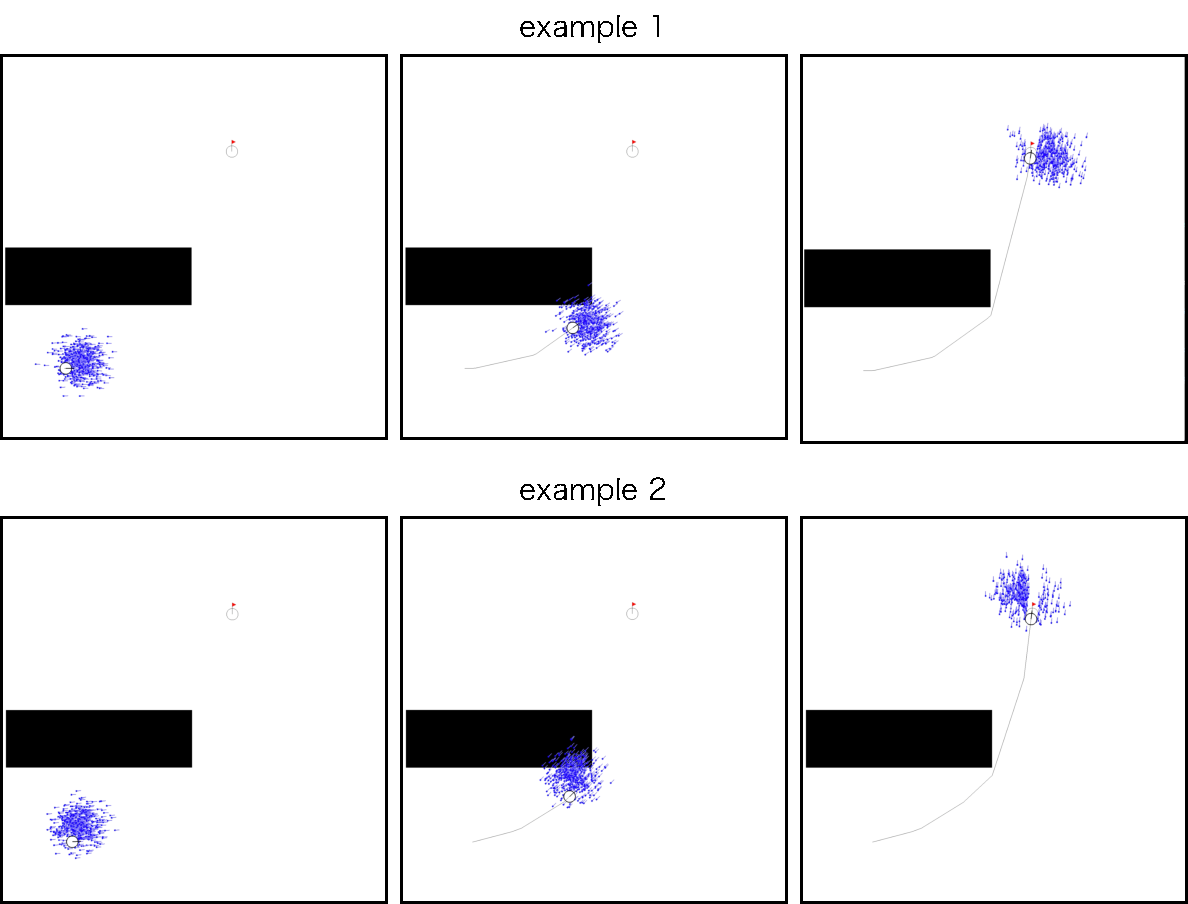
\includegraphics[width=15cm, ]{true_pose.pdf}
    \caption{Robot behavior by true pose}
    \label{fig:true pose}
  \end{center}
\end{figure}

パーティクルの平均姿勢$\bar{\V{x}}$を行動決定に利用した場合、図\ref{fig:average pose}に示すような挙動となる。
パーティクルの初期姿勢は、正規分布に従うノイズによるばらつきがあるため、$\bar{\V{x}}$は分布のほぼ中心に位置する。
図の上部の試行では、ロボットの真の姿勢$\V{x}^{*}$は分布の右下にあるため、障害物付近を通る際アウトコース側を移動する。
したがって、障害物に突入することなくゴールへと向かっている。
一方で、図の下部の試行では、$\V{x}^{*}$がインコース側を移動しているため、障害物に衝突してしまっているのが分かる。

\begin{figure}[H]
  \begin{center}
    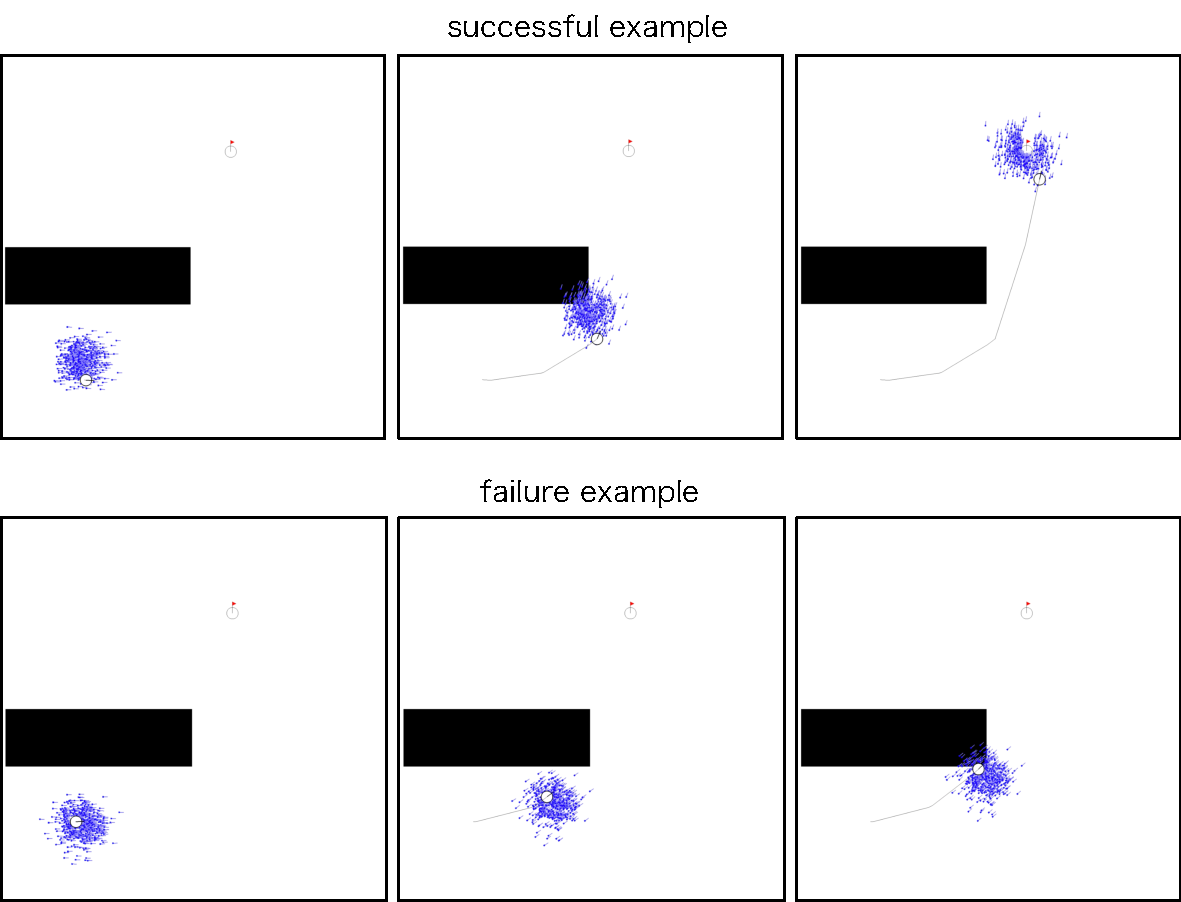
\includegraphics[width=15cm, ]{average_pose.pdf}
    \caption{Robot behavior by particles average pose}
    \label{fig:average pose}
  \end{center}
\end{figure}

続いて、提案手法による動作について確認する。
図\ref{fig:avoid pfc good}に、提案手法による試行の一例を示す。
提案手法では、パーティクル全体が障害物を避けるように移動している。
そして、ゴール周辺へとたどり着いた後、ゴール探索動作を行いタスク成功となっている。
$t=12.7[\si{s}]$でひとつのパーティクルが障害物に入りそうになった際、$m^{(i)}_{\rm avoid}$の値が最大値となる。
ロボットはそのパーティクルの行動を最優先するように右旋回ののち前進し、パーティクルが障害物に侵入するのを防ぐ動作を行った。

\begin{figure}[H]
  \begin{center}
    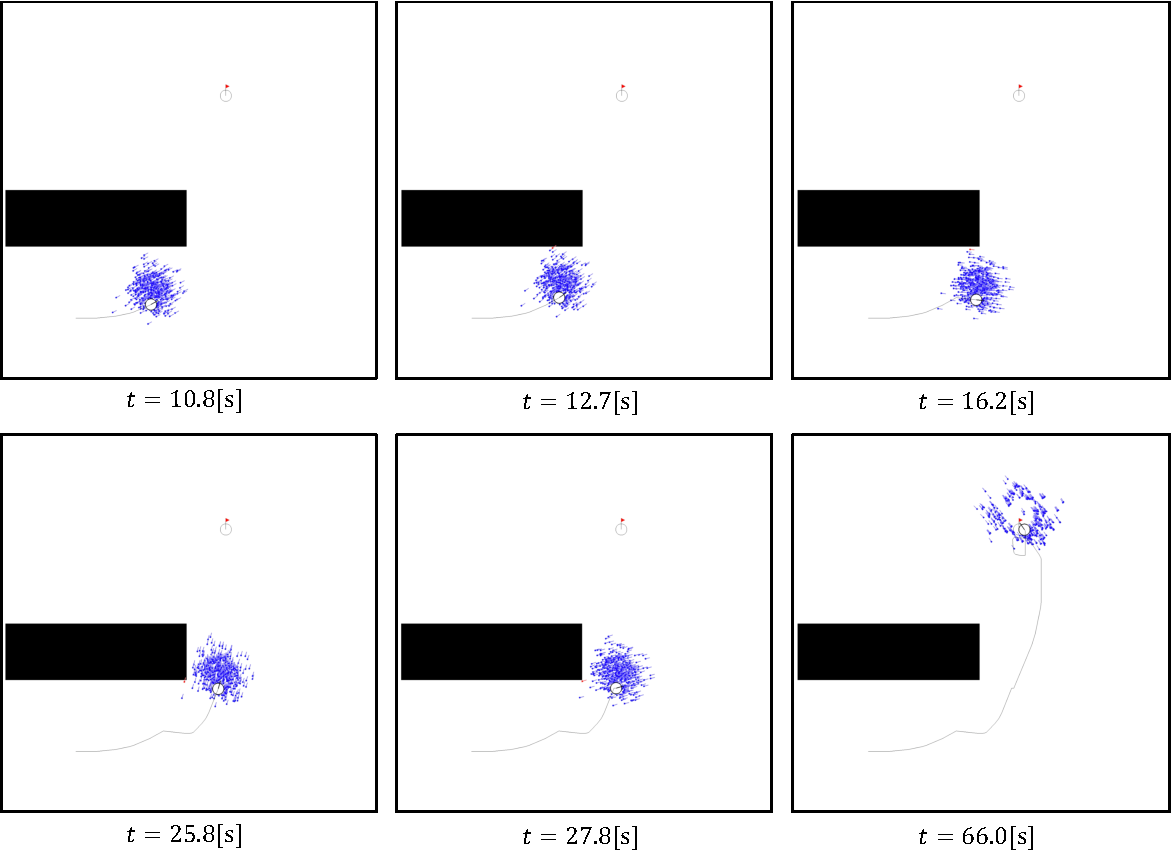
\includegraphics[width=15cm, ]{avoid_pfc_good.pdf}
    \caption{Robot behavior by PFC method with avoidance}
    \label{fig:avoid pfc good}
  \end{center}
\end{figure}

しかし、提案手法の動作には、無駄な動きの多さが伺える。
図\ref{fig:avoid pfc kakukaku}に示す試行は、ロボットの無駄な動作が分かりやすく現れている。
$t=15.3[\si{s}]$でパーティクルが一つ障害物に侵入しそうになり、$t=17.7[\si{s}]$で回避するように動作する。
その後、再度$t=19.8[\si{s}]$で別のパーティクルが障害物に親友しそうになり、$t=12.7[\si{s}]$で回避動作をする。
このように、パーティクルの分布によっては、ゴールへ向かう動作と回避動作が何度も交互に繰り返され、ギザギザの軌跡を描く。

本手法では、次の動作によるパーティクルの報酬のみから、$m^{(i)}_{\rm avoid}$を決定しているため、
このようにその場しのぎのような動作になると考えられる。
これを防ぐためには、数ステップ先の動作までを含んで回避動作を考えるという方法が、有効ではないかと予想される。
しかし、この計算はロボットが動作するリアルタイムで行える必要があるため、計算量と時間の問題が発生すると考えられる。

\begin{figure}[H]
  \begin{center}
    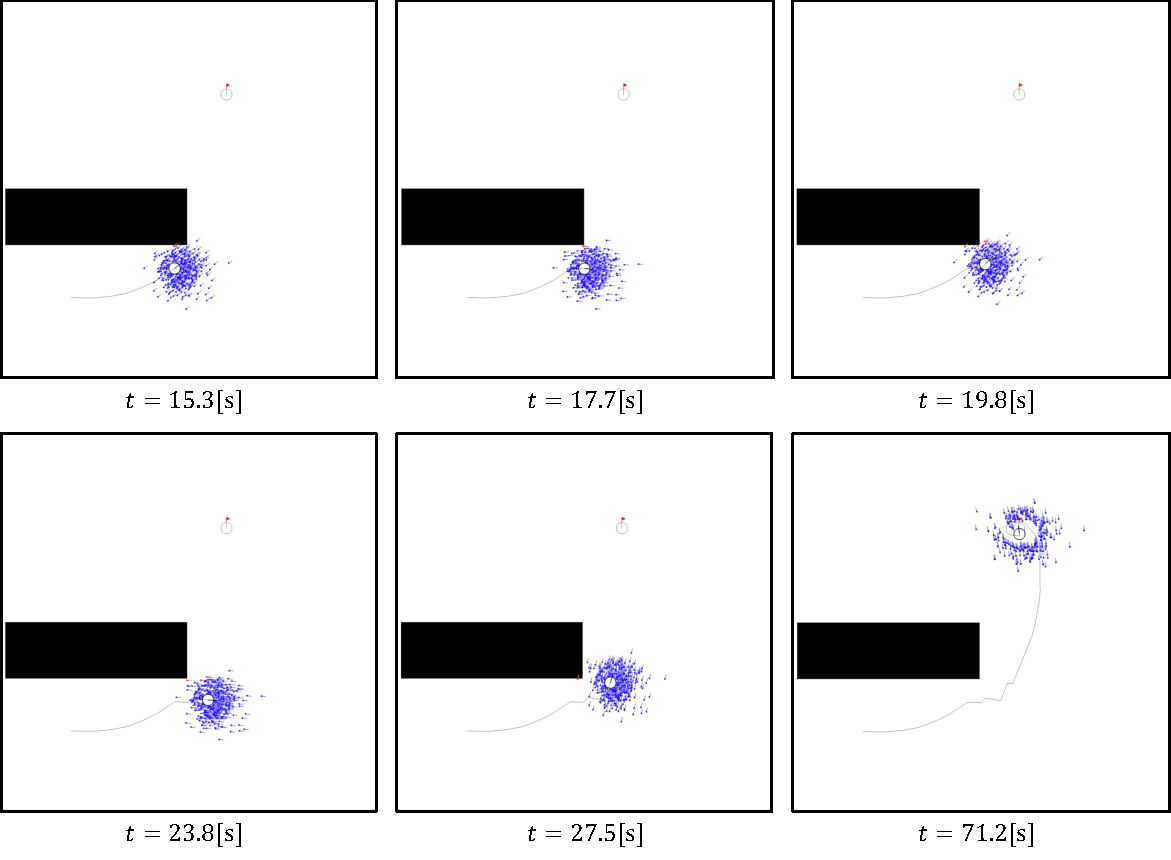
\includegraphics[width=15cm, ]{avoid_pfc_kakukaku.pdf}
    \caption{Robot behavior by PFC method with avoidance}
    \label{fig:avoid pfc kakukaku}
  \end{center}
\end{figure}

最後に、通常のPFC法とQ-MDP法での動作について確認する。
まず、通常のPFC法による動作の様子を、図\ref{fig:pfc}に示す。
図の上段がタスク成功時の動作であり、下段がタスク失敗時の動作である。
通常のPFC方では、分布全体がかなりインコース側を走行し、多くのパーティクルが障害物内を移動しているのが分かる。
成功時と失敗時の違いは、パーティクルの平均姿勢$\bar{\V{x}}$を利用した行動と同様に、真の姿勢$\V{x}^{*}$がアウトコース側に存在しているか否かである。
成功時の右のコマでは、障害物を回避することに成功したのち、ゴールを探索する動作を行いタスク成功したことが分かる。

\begin{figure}[H]
  \begin{center}
    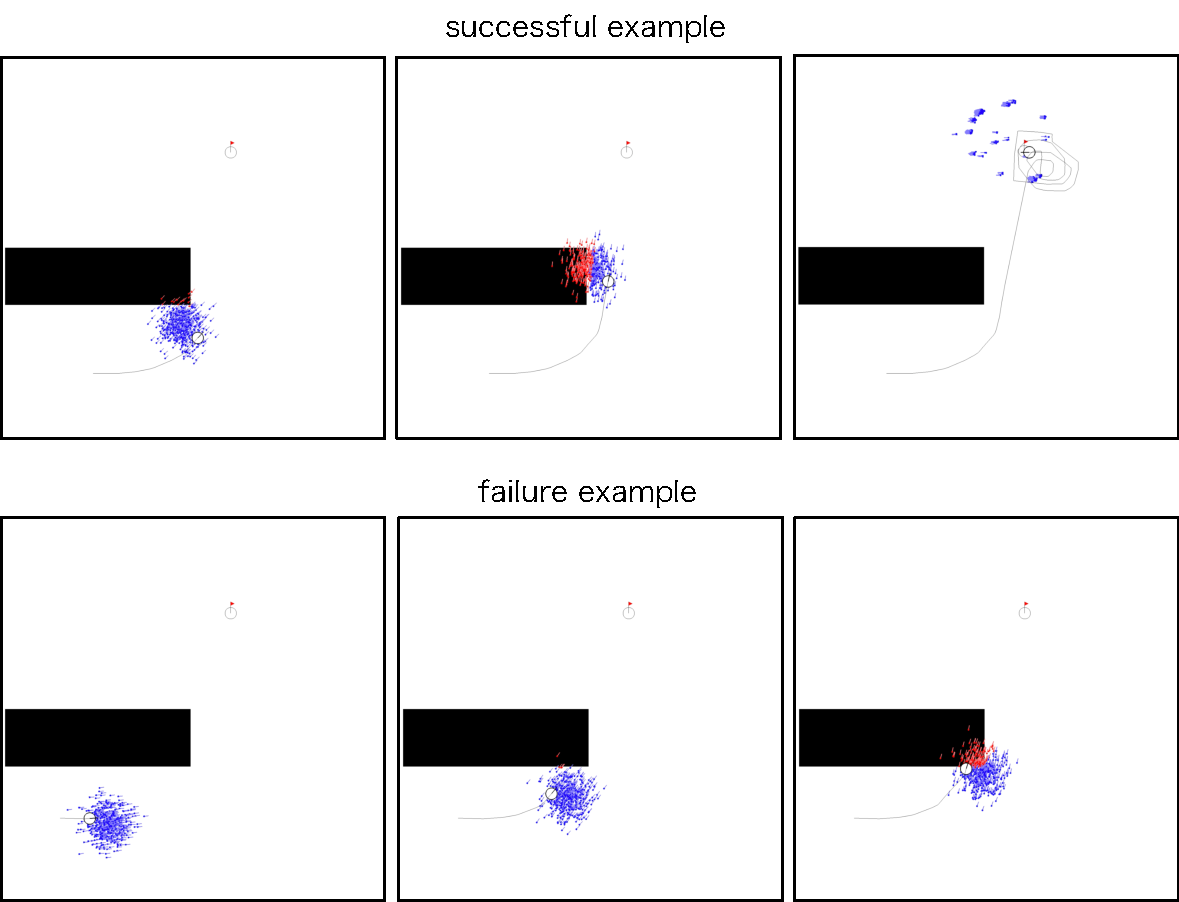
\includegraphics[width=15cm, ]{pfc.pdf}
    \caption{Robot behavior by normal PFC method}
    \label{fig:pfc}
  \end{center}
\end{figure}

Q-MDP法の動作については、図\ref{fig:q-mdp}に示す。
上段のタスク成功時の動作と下段のタスク失敗時の動作ともに、いくつかのパーティクルは障害物内を移動しているものの、
大部分は障害物を回避するような動作を行っている。
障害物を回避後は、ゴールへと向かう。
成功時の動作では、分布の中央付近に$\V{x}^{*}$が存在しているため、ゴールへ入ることができている。
しかし、Q-MDP法はゴールの探索動作を行わないため、失敗時の動作ではゴール付近で行動が長時間停滞し失敗となる。

\begin{figure}[H]
  \begin{center}
    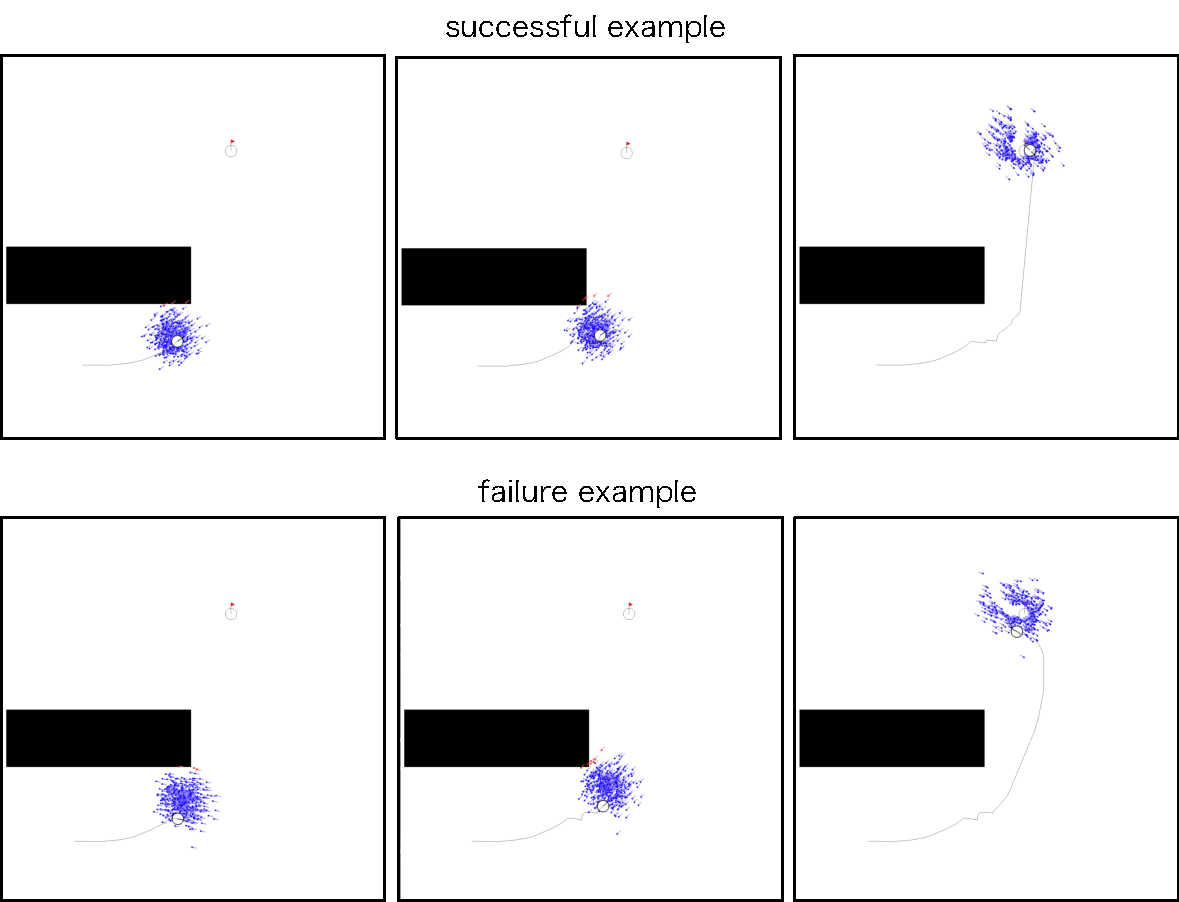
\includegraphics[width=15cm, ]{q-mdp.pdf}
    \caption{Robot behavior by Q-MDP method}
    \label{fig:q-mdp}
  \end{center}
\end{figure}

%%%%%%%%%%%%%%%%%%%%%%%%%%%%%%%%%%%%%%%%%%%%%%%%%%%%%%%%%%%%%%%%%%%%%%%%%%%%%%%%
% \section{考察} \label{section:考察}

\chapter{結論} \label{chapter:conclusion}

%%%%%%%%%%%%%%%%%%%%%%%%%%%%%%%%%%%%%%%%%%%%%%%%%%%%%%%%%%%%%%%%%%%%%%%%%%%%%%%%
\section{本論文のまとめ}
本論文では、自己位置推定の不確かさを考慮した障害物の回避行動を自律移動ロボットに行わせるための手法を提案した。
MCLによって自己位置推定を行うロボット用に、信念分布を近似するパーティクルの分布全体が、障害物を回避するような動作を生成した。
この動作は、行動決定に与える影響度を決定するパラメータを各パーティクルに持たせ、この数値をタスク実行中に動的に変化させることで実現した。
次の行動で障害物に侵入するパーティクルの数値を大きくし、障害物を避けようとする動作を強めることで、目的の動作を達成した。

また、提案手法の有効性について、先行研究と比較し評価した。
既存の手法では、障害物内をパーティクルの分布が移動することにより、ロボットの障害物への衝突が起こる可能性があることを示した。
提案手法は、パーティクルの分布が障害物内を移動するのをなくしたことで、この衝突の可能性を大幅に減らすことに成功した。

他にも、本論文で提案した手法では、ロボットの挙動に無駄があることが問題と述べた。
移動ロボットが障害物を回避するとき、ギザギザの軌跡を描くように動作する。
これは、パーティクル一つが障害物に入っただけで、動作が大きく変わりすぎるためだと考えられる。


%%%%%%%%%%%%%%%%%%%%%%%%%%%%%%%%%%%%%%%%%%%%%%%%%%%%%%%%%%%%%%%%%%%%%%%%%%%%%%%%
\section{今後の展望}
今後、ロボットの挙動の無駄の多さについて改善する必要があると言える。
これは、今回新たに導入した、パーティクルが行動決定に与える影響度の増やし方を工夫することで実現できる可能性がある。
現在の手法では、パーティクルが一つでも障害物に侵入しそうになった場合、影響度を一気に最大にしている。
これを徐々に増加させていくように変更する方法が一つ考えられる。
また、パーティクルの数から、次の行動でロボットが障害物に衝突する確率が計算できる。
この確率に応じて、ロボットの行動を徐々に回避動作へと移行させるように、パラメータを増加させていくことも、有効であると考えられる。

今回の評価実験のような、ゴールと障害物が遠くに存在している環境では、
障害物の回避を行うフェーズとゴール探索動作を行うフェーズが分かれている。
しかし、ゴール付近に障害物が存在する場合、障害物回避動作とゴール探索動作はトレードオフとなり、
2つの動作をループするようなデッドロックが発生する可能性があると考えられる。
そういった場合、障害物への衝突確率を判断材料に、行動を回避動作から探索動作へ徐々に移行させていくような方法が有効ではないかと考えられる。
また、パラメータの最大値も各パーティクルに個別で持たせることで、
障害物に入りそうになる度に、行動へ与える影響度が大きくなりにくくなるような方法も、有効ではないかと考えられる。


%%% 参考文献 %%%
% よほどのことが無い限りet al.は使わないことにしましょう
\bibliographystyle{jualpha}
\bibliography{./references}

\newpage
\printindex

\end{document}
